%%%%% %%
%% Sample document ``thesis.tex''
%%
%% Version: v0.2
%% Authors: Jean Martina, Rok Strnisa, Matej Urbas
%% Date: 30/07/2008
%%
%% Copyright (c) 2008-2011, Rok Strniša, Jean Martina, Matej Urbas
%% License: Simplified BSD License
%% License file: ./License
%% Original License URL: http://www.freebsd.org/copyright/freebsd-license.html
%%%%%

% Available documentclass options:
%
%   <all `report` document class options, e.g.: `a5paper`>
%   withindex   - enables the index. New index entries can be added through `\index{my entry}`
%   glossary    - enables the glossary.
%   techreport  - typesets the thesis in the technical report format.
%   firstyr     - formats the document as a first-year report.
%   times       - uses the `Times` font.
%   backrefs    - add back references in the Bibliography section
%
% For more info see `README.md`
\documentclass[withindex,glossary]{cam-thesis}

% Citations using numbers
\usepackage[numbers]{natbib}
\usepackage{todonotes}
\usepackage{enumerate}

%%%%%%%%%%%%%%%%%%%%%%%%%%%%%%%%%%%%%%%%%%%%%%%%%%%%%%%%%%%%%%%%%%%%%%%%%%%%%%%%
%% Thesis meta-information
%%

%% The title of the thesis:
\title{Towards Provenance as a First Class Construct of \\
Dependable Computing Systems}

% Alternate titles
% Provenance based trustworthiness assessment in computing systems

%% The full name of the author (e.g.: James Smith):
\author{Nikilesh Balakrishnan}

%% College affiliation:
\college{Churchill College}

%% College shield [optional]:
% \collegeshield{CollegeShields/Christs}
\collegeshield{CollegeShields/Churchill}
% \collegeshield{CollegeShields/Clare}
% \collegeshield{CollegeShields/ClareHall}
% \collegeshield{CollegeShields/CorpusChristi}
% \collegeshield{CollegeShields/Darwin}
% \collegeshield{CollegeShields/Downing}
% \collegeshield{CollegeShields/Emmanuel}
% \collegeshield{CollegeShields/Fitzwilliam}
% \collegeshield{CollegeShields/Girton}
% \collegeshield{CollegeShields/GonCaius}
% \collegeshield{CollegeShields/Homerton}
% \collegeshield{CollegeShields/HughesHall}
% \collegeshield{CollegeShields/Jesus}
% \collegeshield{CollegeShields/Kings}
% \collegeshield{CollegeShields/LucyCavendish}
% \collegeshield{CollegeShields/Magdalene}
% \collegeshield{CollegeShields/MurrayEdwards}
% \collegeshield{CollegeShields/Newnham}
% \collegeshield{CollegeShields/Pembroke}
% \collegeshield{CollegeShields/Peterhouse}
% \collegeshield{CollegeShields/Queens}
% \collegeshield{CollegeShields/Robinson}
% \collegeshield{CollegeShields/Selwyn}
% \collegeshield{CollegeShields/SidneySussex}
% \collegeshield{CollegeShields/StCatharines}
% \collegeshield{CollegeShields/StEdmunds}
% \collegeshield{CollegeShields/StJohns}
% \collegeshield{CollegeShields/Trinity}
% \collegeshield{CollegeShields/TrinityHall}
% \collegeshield{CollegeShields/Wolfson}
% \collegeshield{CollegeShields/FitzwilliamRed}

%% Submission date [optional]:
% \submissiondate{November, 2042}

%% You can redefine the submission notice [optional]:
% \submissionnotice{A badass thesis submitted on time for the Degree of PhD}

%% Declaration date:
\date{September, 2017}

%% PDF meta-info:
\subjectline{Computer Science}
\keywords{Provenance Dependable Assurance}



%%%%%%%%%%%%%%%%%%%%%%%%%%%%%%%%%%%%%%%%%%%%%%%%%%%%%%%%%%%%%%%%%%%%%%%%%%%%%%%%
%% Abstract:
%%
\abstract{%
\begin{itemize} 
\item Provenance capture in computing systems.
\item Use of provenance to reason about computations in the context of control flow and data flow.
\item We provide real implementations of systems that allows us to track computations in the context of scientific computing.
\item We also provide a prototype implementation of tracing data flow in the context of disk I/O, from the application to the device and back.
\end{itemize}
}



%%%%%%%%%%%%%%%%%%%%%%%%%%%%%%%%%%%%%%%%%%%%%%%%%%%%%%%%%%%%%%%%%%%%%%%%%%%%%%%%
%% Acknowledgements:
%%
\acknowledgements{%
  Add acknowledgements here ...
}



%%%%%%%%%%%%%%%%%%%%%%%%%%%%%%%%%%%%%%%%%%%%%%%%%%%%%%%%%%%%%%%%%%%%%%%%%%%%%%%%
%% Glossary [optional]:
%%
\newglossaryentry{HOL}{
    name=HOL,
    description={Higher-order logic}
}



%%%%%%%%%%%%%%%%%%%%%%%%%%%%%%%%%%%%%%%%%%%%%%%%%%%%%%%%%%%%%%%%%%%%%%%%%%%%%%%%
%% Contents:
%%
\begin{document}

%%%%%%%%%%%%%%%%%%%%%%%%%%%%%%%%%%%%%%%%%%%%%%%%%%%%%%%%%%%%%%%%%%%%%%%%%%%%%%%%
%% Title page, abstract, declaration etc.:
%% -    the title page (is automatically omitted in the technical report mode).
\frontmatter{}



%%%%%%%%%%%%%%%%%%%%%%%%%%%%%%%%%%%%%%%%%%%%%%%%%%%%%%%%%%%%%%%%%%%%%%%%%%%%%%%%
%% Thesis body:
%%
\chapter{The Need For Provenance}

\section{The Problem}
\begin{itemize}
\item Computing has become ubiquitous and pervasive.
\item Generation of large amounts of data.
\item More computing performed and decisions taken based on this data.
\item These results are then used in all aspects of society: Business, Science, Social and Government.
\item Business example from insurance, banking and e-commerce. Link real articles.
\item Examples from scientific computing, look at papers on cancer research etc. Look for other research that publishes results on data.
\item These computations are much more interleaved and used by each other. Take for example the 2008 debt crisis:
\item Financial products were created on top of other financial products and derivatives and new products where nobody understood
what they were actually representing. c.f. when people took on the product they did not understand the risk they were actually taking on.
\item Impact of these computations is huge. If the computation is wrong or inaccurate, it can have a huge impact on the structure of
society and/or have huge social, scientific, societal implications. Examples: e.g. Climate change controversy, Argentina Debt Crisis,
2008 Wall Street Crash etc.
\end{itemize}

\section{The Hypothesis}
\begin{itemize}
\item It is possible to build abstractions that allow people to track the inputs, operations and outputs of a computation
(provenance of a computation) so that you can reason about it from both a time and space perspective as you use the data
produced by the computation.
\item Having this support will allow us to mitigate the trust issues that arise from non-ascertainable computations.
\end{itemize}


\section{Thesis outline}
\begin{itemize}
\item In this thesis I explore the fundamental primitives required to build systems that offer provenance as a first-class construct
of systems.
\item To this end I focus on two systems:
(i) OPUS: A system for adding data and computational provenance support for scientific computational pipelines.
(ii) NORAD: Non-repudiable assertions for disk I/O. NORAD is a system that provides assurances about the trusworthiness of data in a computational system.
\item For each of these systems I provide real-world engineering systems and outline the design-space, implementation and use-cases for these systems.
\item I conclude by offering a look into further directions.
\end{itemize}

\section{Contributions}
The contributions of this thesis are thus:
\begin{itemize}
\item Design and implementation of a provenance system called OPUS, for scientific workloads.
\item Tools and applications that utilise this system to show its utility in the context of scientific computation.
\item A performance characterisation of the system compared to existing systems.
\item A prototype system, NORAD for asserting the data provenance captured by provenance systems.
\item A characterisation of NORAD's performance and use-cases showing its utility.
\end{itemize}

\chapter{A Background into Provenance}
This chapter presents the background literature in the area of provenance.
\begin{itemize}
\item What is provenance and what is the use of provenance? A systematic capture of meta-data that describes the where, when and how of data and computations.
\item Meta-data is typically a graph that describes relationships between various elements or entities in a system that contributed to a piece of data produced by the system.
\item How is it captured?
\item Brief introduction into the various capture approaches used, system, workflow, database, etc. Our interest is in providing this support at the system level.
\item Therefore we focus on those mechanisms that capture provenance at the system call, filesystem and OS layers.
\item Introduce the concept of granularity of capture, the layer at which the capture happens and what the provenance describes at each layer of abstraction.
\item How provenance can be queried and used?
\item What about the security of the provenance itself? Current state-of-art in provenance security is the SPROV work that ensures the integrity and authenticity if provenance records once its captured.
\item What about provenance that was circumvented or falsified at the point of capture?
\item Cite the Primer on Provenance paper.
\end{itemize}

\chapter{OPUS: Provenance Support for Scientific Workloads}
The work described in this chapter is a joint contribution with Thomas Bytheway. My primary contribution in this body of work is as follows:

\begin{itemize}
\item Equal intellectual contribution with Thomas Bytheway in the system design of OPUS.
\item Participated and contributed in the discussions on PVM, especially in modelling corner cases using PVM.
\item Implemented most of the interposition mechanism in the OPUS front-end.
\item Re-implemented parts of the OPUS backend to work with a graph database store, Neo4J.
\end{itemize}

\section{Introduction}
In ~\ref{ch:two} we have seen previous approaches for provenance capture, query and some real-world use-cases for provenance. In this chapter we attempt to outline the shortcomings of existing provenance systems, detailing the problems as the motivation for the design and implementation of OPUS, a user-space provenance capture, analysis and query tool for scientific computing. We show that it is possible to build tools and applications that can use this provenance captured to aid in tracking, archiving and debugging of multi-step ad hoc scientific computations.

\section{Motivation}
Today most physical sciences are computation based.
At its core, scientific computations involve the development of models and simulations to understand the natural world. 
These models and simulations are typically composed of multiple computational steps where data is input and output within each step, forming an experiment pipeline wherein data output in a step is used as input in the next step.
Once a result is obtained and interpreted, confidence in the result is obtained by analysing, repeating and reproducing the experiment independently.
In order to do this scientists have traditionally used manual and ad hoc techniques to record the data inputs and contexts (parameters, configuration, dependencies etc.) used in the computations to produce the result.
This manual process is however prone to errors and often not complete, resulting in experiments not being reproducible ~\cite{non-rep, nature}. 
Provenance systems ~\cite{PASS, BURRITO, StoyBook} in the past have attempted to automate this effort and ease the process of reproducibility by automatically tracking data and computation.
However, these systems have lacked adoption in the real-world and have merely resulted in being research or experimental prototypes.
This is primarily because these systems are not widely available or easily deployable in practice.
Most of these systems require changes to existing workflows, require modification to the underlying OS or require the use of specialised systems.
Our goal is to design and implement a lightweight, general purpose provenance system that has a minimum barrier to entry, especially in the context of scientific computing.
To this end, we have designed OPUS, a provenance system that is designed to work entirely in user-space and is based on several key design constraints discussed in the next section ~\ref{sec:constraints}.

\section{A unique constraint space}
OPUS draws inspiration from previous approaches in building general purpose provenance systems but addresses several of their shortcomings outlined in ~\ref{sec:opusmotiv}. The design of OPUS is based on the following requiements:

\begin{itemize}

\item \textbf{Non-intrusiveness:}
It is our observation that most computational scientists seldom have \texttt{root} or system level access to install and update software. Therefore it is important for a general purpose system to be as non-intrusive as possible i.e. the system should not require changes to the underlying OS or the use of bespoke kernel modules to capture provenance. Therefore a major design principle for OPUS is that it must work entirely in user-space. An added advantage of designing OPUS to work in user-space is that it becomes easier to ensure that in a shared system, users of OPUS do not affect other users in the system.

\item \textbf{Ease of installation:}
In addition to being non-intrusive a general purpose provenance system must be easy to install. The installation must be self-contained, having no external dependencies and requiring minimal configuration changes. This ensures that the barrier to adoption of such systems by users such as scientists is as low as possible.

\item \textbf{Seamlessness:}
Scientific computing across disciplines are diverse in terms of the workflow used, therefore a general purpose provenance system should not require the users to modify their existing workflow in order to use the system. OPUS should therefore be designed to drop into a user's environment and seamlessly integrate with existing workflows and capture provenance.

\item \textbf{Low overheads:} 
Scientific applications are typically executed multiple times and each run can perform multiple iterations until the computation converges to a specific expected result. This execution could therefore take anywhere from seconds to minutes to hours depending on the complexity of the computation performed. Therefore it is important that a provenance system like OPUS impose minimal overheads on the application run time. Similarly, the application could be executing in memory and storage constrained environments, therefore keeping the spatial overheads low is also a useful property to consider while designing the system.

\item \textbf{Completeness:} 
Existing systems record only a subset of operations applications perform on files and processes. This restricts the range of provenance queries that one can implement. To support a richer set of queries OPUS should be designed to capture all file and process relatede operations. Also, merely capturing file and process interactions ignores the execution context (library versions used, command line parameters used, environment variables etc.) in which these operations were done. Therefore the mechanism OPUS uses should capture the surrounding execution context as well. 

\item \textbf{Reasoning about provenance:}
The ultimate goal of capturing provenance is to use it to reason about application execution and data used or produced. However, provenance is itself represented and stored as data, therefore we require a structured mechanism to reason about provenance data as it is recorded and stored. Existing systems are either rigid or use ad-hoc approaches to record and store provenance. In order for provenance to be useful and effective, we require a more formal approach to reason about the provenance data itself. In section ~\ref{sec:pvm} we discuss PVM, a semi-formal model for generating and representing provenance.

\end{itemize}

\section{Design Decisions} 
The design of OPUS is guided by the requirements outlined in ~\ref{sec:constspace}.
The initial design is intended for on-host provenance capture, analysis and query.
In this section we discuss our approach and some of the decisions involved in designing OPUS.


\subsection{Provenance Capture}
One of the main components in the design of OPUS is the provenance capture component.
In the context of scientific computing, our requirement for OPUS is to employ a seamless, non-intrusive, always-on and lightweight method for provenance capture.
To build such a system we explore several existing mechanisms to capture provenance.
A key observation here is that most of these mechanims have conventionally been used in tracing and debugging applications.
Since the data captured by these techniques overlaps to a considerable amount with the data required for provenance we can leverage these mechanisms to build provenance systems.

\paragraph{FUSE} is a framework that allows non-privileged users to implement a custom filesystem in user-space. FUSE consists of (i) a kernel module which registers a filesystem with the kernel's virtual file system (VFS) and (ii) a user-level daemon that either implements the entire filesystem functionality or acts as a pass-through layer to a kernel filesystem. A proof-of-concept system ~\cite{StoryBook} has shown that it is possible to use this framework to capture I/O activities of applications and can be done without any modification to the application or existing workflows as perceived by the user. Therefore for OPUS, FUSE is a viable option for provenance capture. However, the use of FUSE for provenance capture has several limitations:
(i) FUSE requires root permissions to install and configure.
(ii) With certain workloads FUSE can impose a significant overhead on application I/O ~\cite{StoryBook}.
(iii) FUSE only intercepts I/O activities, other crucial process level operations required to build more richer provenance is not visible to FUSE.

\paragraph{PTrace} is a process tracing functionality supported on most Unix-like OSes. 
PTrace allows a tracer process to trace the execution of a target process.
When an event of interest (for example system calls) is executed by the target, the underlying OS stops the execution of the traget and switches control to the tracer process.
The tracer process can then examine the register and memory state of the target process.
This is the core mechanisms used to implement debuggers.
This can be a useful technique to capture provenance as well since it provides complete visibility into the target program's execution.
The primary advantage of using PTrace for provenance capture is that is does not require root permissions unless the target process is executing as root.
However, PTrace imposes a high temporal overhead (~30\%) on the process being traced since the mechanism requires multiple context switches for each event being traced.
This makes PTrace impractical for use in an always-on, system-wide provenance capture system.

\paragraph{Kernel-level Tracing:}
Over the years systems developers have recognised the need for a flexible tracing infrastructure for both the kernel and user-space applications.
A number of mechanisms and tools ~\cite{DTrace, SystemTap, Uprobes, LXCModules} have been created to support this requirement.
The core idea with these mechanisms is to provide support in the kernel to trace application activity, typically by monitoring the interaction of the application with the OS.
The key benefits of kernel-level tracing mechanisms are that it is completely seamleass to applications, executes at a higher privilege level and therefore potentially secure from user-space attacks.
A user will require \texttt{root} permissions to enable or configure these tracing mechanisms.
However, the main limitation of using such an approach for provenance capture is that most of these mechanisms have been introduced fairly recently and they may not be supported in older kernel versions.
Given that our requirement is to support scientific workloads our initial decision is to not use such techniques for provenance capture.


\paragraph{Binary Rewriting} is the process of transforming an application binary by modifying individual instructions to implement a specific functionality while still retaining the semantics of the original application. 
Binary rewriting can happen either (i) statically, where the application binary is disassembled and the instructions are modified or (ii) dynamically, where the instruction stream is modified at runtime using just-in-time compilation. 
Provenance capture can be implemented using such mechanisms wherein specific instructions (for e.g. syscall instruction) executed by the application are intercepted and captured.
Manually implementing this correctly and in a generic manner is a difficult exercise, however, there are a number of tools and frameworks ~\cite{PIN, DynInst} that can significantly ease this process.
Given that this mechanism can be implemented entirely in user-space it can be considered a viable method for provenance capture for a system like OPUS.
However, for the initial design our goal is to use a quicker approach for prototyping the system, therefore binary rewriting may not be the ideal choice to implement the capture component.

\paragraph{LD\_PRELOAD:} is a feature provided by the runtime linker that enables overriding of symbols in libraries linked by programs at load time. In order to override the symbols, a new library with definitions for the symbols to be overridden must be implemented and the environment variable LD\_PRELOAD set to this library path. In the context of provenance capture we can use this mechanism to interpose calls made by applications to the standard C library. Given that the standard C library is a wrapper over the system call interface, this becomes a viable method for capturing provenance at system call granularity.
The primary advantages of the LD\_PRELOAD mechanism is that (i) it imposes a much lower overhead when compared to other user-space system call interception mechanisms and (ii) it is easier to implement and prototype since there is no special API or interface required to implement it.
However, LD\_PRELOAD assumes that applications link with the standard C library dynamically and that system calls are always invoked by application via the C library.
For a system that captures provenance in the context of scientific computing it is reasonable to assume that most programs dynamically link with and interface with the OS using the C library. Given that this mechanism satisfies a majority of the requirements for a lightweight, userspace provenance capture system, our decision for the first version of OPUS is to employ library interposition as a method for provenance capture.


\subsection{Provenance Analysis} 
The raw provenance stream consisting of system call event data from executing programs should be converted to a meaningful representation that describes the provenance of processes, files, sockets etc.
In previous general purpose provenance systems ~\cite{PASS, PASSv2} this has been represented as a directed acyclic graph (DAG) where the nodes represent entities such as processes and files while the edges describe the interation between these entities as shown in figure xxx.\todo{Show a simple DAG of processes and files}
OPUS uses a similar approach and collects event streams from processes executing on the machine and converts it into a provenance graph.
However, unlike previous systems, OPUS uses a semi-formal model, PVM (Provenance Versioning Model) to map and model the undelying system semantics.
PVM formalises the process by which entities in the graph are updated and allows us to reason about changes to these entities.
PVM is discussed in detail in section~\ref{sec:PVM}

\paragraph{On-host or Off-host analysis?}
The provenance analysis component of OPUS can run on the same host where system call events are captured or off-host, on a dedicated server.
Our initial design assumes that all event streams from a single host will be handled by an analyser instance dedicated for that host.
However, given the context of scientific computing our goal is to make OPUS easy to adopt and minimise the barrier to entry, to this end our initial version of OPUS will run the analysis component on the same host where capture is performed.

\paragraph{Event Ordering:}
Maintaining a correct view of order of events in the system is important for provenance systems since small changes in the order of events can produce significant semantic changes to the graph being generated.
For example, consider two events in the system, event \texttt{E1} where a process \texttt{P1} opens a file \texttt{F} to write to it and another event \texttt{E2} wherein a process \texttt{P2} unlinks \texttt{F}.
In such situations, processing events in the correct order is crucial in order to reflect the actual side-effects these operations have on the underlying system.

A naive approach to implement ordering is to use the system clock to timestamp events.
However, the system clock for a given machine is not guaranteed to be sane over any period due to NTP updates or users manually changing the system time.
Therefore using the system clock is not a reliable method to order events.
A more reliable approach is to use the machine's hardware monotonic clock as it provides the guarantee of a consistent increasing time value over any single run of a given machine.
With the initial version of OPUS we favour this approach, especially since we plan to run a dedicated instance of OPUS on-host.

\subsection{Provenance Storage}
Once the raw system call events are received by the OPUS backend and transformed into provenance using PVM rules, it must be persisted in a suitable data store.
As part of the design we consider primarly three types of data stores:

\paragraph{Relational:} 
Relational databases have been around for decades and are the database of choice for many data-intensive storage and retrieval applications.
Most relational databases support SQL as the standard language for queries and this makes transitioning between various implementations of relational databases much easier.
However, given the graph structure of our provenance data, expressing traversal queries for relational data can result in exceedingly complex queries.
At the time of designing OPUS there was a lack of support for hierarchical queries in SQL therefore relational databases was not first choice for our data store.
Today, there is support for Common Table Expressions (CTEs) which allow us to effeciently express complex traversal queries in relational databases.
For the initial implementation of OPUS we need to ensure that the data is easily storable and retrievable for the purposes of tracking scientific data and computation, therefore relational databases may not be the best fit for our needs.

\paragraph{Key-Value:}
Key-Value databases have gained popularity in recent times mainly because they are schemaless and simple to use. They and desgined for storing, retrieving and managing associative arrays.
KV stores are avialable for a range of applications from heavy weight distributed systems to single node systems running as an embedded database instance within applications.
Previous general purpose provenance systems such as PASS have shown that it is possible to use key-value stores ~\cite{BerkleyDB} for the storage and retrieval of provenance.
During the design and implementation of OPUS we've explored the use of LevelDB an embedded key-value store by modelling nodes and edges in the provenance graph to fit the key-value paradigm.
We've observed that although key-value stores are simple to integrate with and use, they have several downsides while modelling provenance graph structured data:
(i) The implementation of features like node and edge types in key-value stores requires partitioning of the key space to encode type information.
(ii) Indexes on node and edge properties have to be manually implemented as key-value stores inherently do not support indexes.
(iii) They do not provide support for an expressive query language such as SQL. Instead, graph traversal queries must be implemented manually at the application layer. This results in an increased number of round-trips to the database and back, leading to a reduction in performance.

Given these shortcomings, our conclusion is that key-value stores are not the best fit for the first phase of OPUS.

\paragraph{Graph:} 
Graph databases can represent our provenance object and relationships more naturally and effectively.
Most graph databases also allow for powerful querying capabilities either via a query language such as Cypher ~\cite{Cypher}  or a traversal API ~\cite{Gremlin}.
For the initial design and implementation of OPUS our requirement is to use a lightweight and easily administerable graph database, while also providing the possibility of scaling the database in future if required.
Given this constraint our decision is to use an embedded Neo4J database to run as part of the OPUS backend (Provenance Analyser) to persist provenance data.
Neo4J also provides the option to scale out to running a dedicated server instance or to cluster several instances if necessary.
This augurs well for our future requirements as well.

\section{System Design}
In this section we describe the system architecture of OPUS and the high level implementation details of each component of the system.

\begin{figure}[t!]
  \centering
    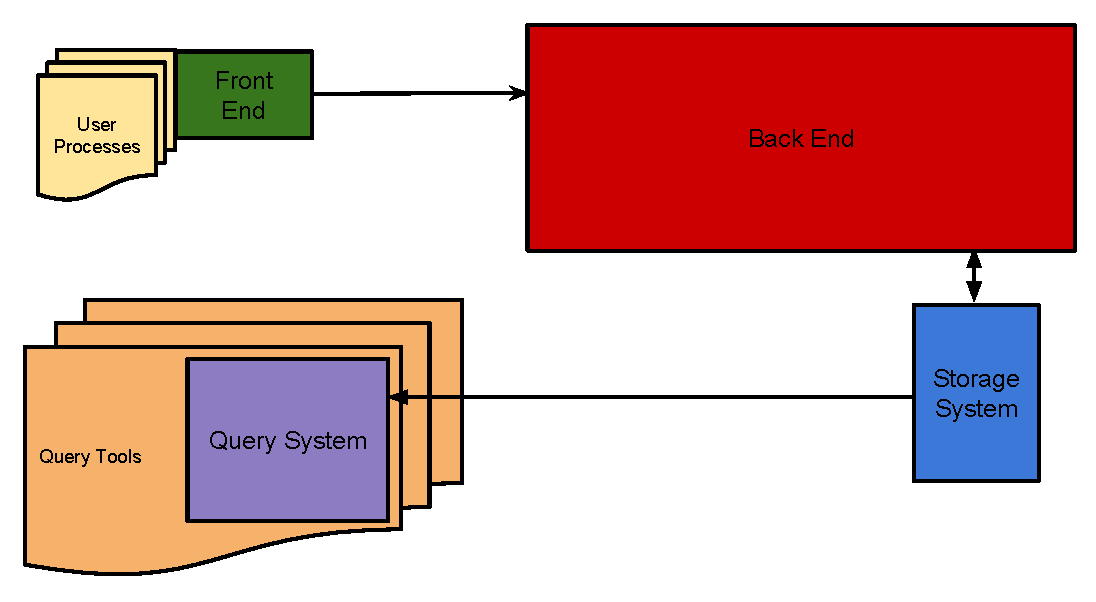
\includegraphics[width=1.0\columnwidth]{BroadProvDesign}
  \caption{OPUS: High Level Design}
  \label{fig:opushld}
\end{figure}

As shown in figure ~\ref{fig:opushld} OPUS consists of four main components:
\begin{itemize}
\item A frontend that captures raw event data from user activities.
\item A backend that analyses the raw event data and transforms them into a provenance graph.
\item A storage system that persists provenance objects and their relationships.
\item A query API that allows users to retrieve the provenance of their data and computations.
\end{itemize} 

The design of the system allows for multiple frontend instances to simultaneously transmit their event stream to the backend for analysis and storage.
%The initial implementation of the system for use in the context of scientific computing will use libc interposition for the events stream capture.
%Other producers using a different method for capturing event streams, for example kernel level instrumentation can easily be plugged into the system if necessary.
The backend for the initial phase comprises of a single analyser instance running on-host converting raw event streams into provenance.
However, the design can be extended to add multiple analyser instances to load balance or handle events from multiple hosts.
The storage system is also pluggable and the design allows this component to be changed in future releases.

\subsection{System Assumptions}
The current implementation of OPUS targets the x86 and x86\_64 processor architectures.
However, the design of OPUS itself is not machine or hardware dependent and can be easily ported to work on other architectures.
We assume that most applications, specifically scientific applications interact with the OS via libc and that that direct invocation of system calls are absent or rare.
Finally, we also assume that most scientific applications dynamically link with libc as the intersposition mechanism relies on the runtime linker.

\subsection{Module Level Desgin}

\begin{figure}[t!]
  \centering
    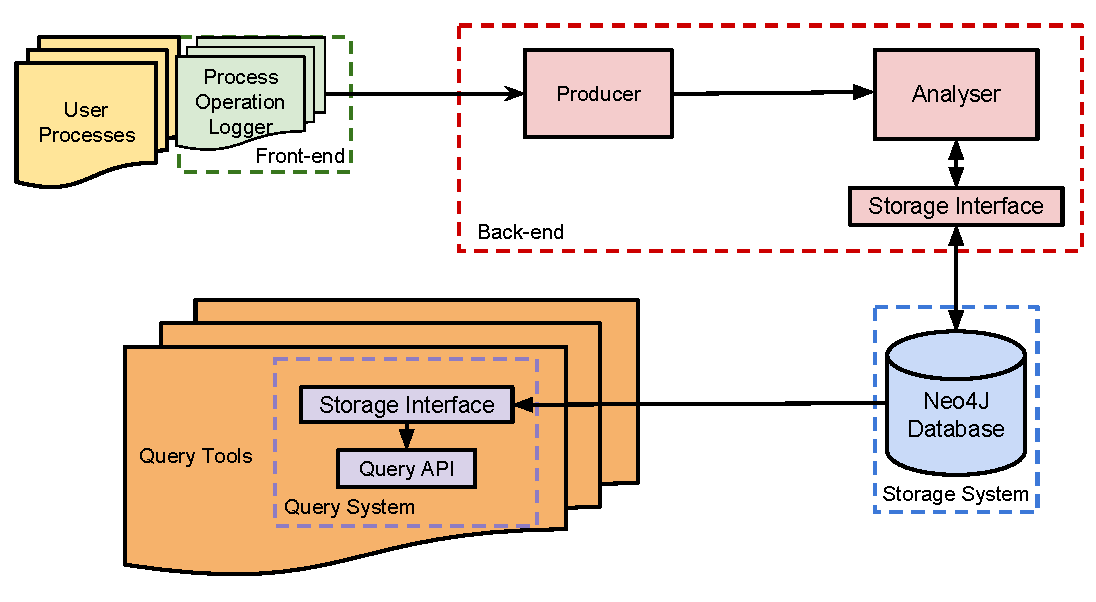
\includegraphics[width=1.0\columnwidth]{ProvDesign}
  \caption{OPUS: Module level design}
  \label{fig:opuslld}
\end{figure}

As shown in ~\ref{fig:opuslld} the primary modules in OPUS consists of a interposition module, connection manager, provenance analyser, storage interface and a graph database.
We now describe implementation details for each of these modules:

\subsubsection{Interposition Module}
The interposition module is a shared library implemented in C++.
This library is loaded transparently on program startup by setting the LD\_PRELOAD environment variable to point to the interposition library path.
Once this is done, when the program binary is loaded into memory, the runtime linker overrides the symbol table with the symbols defined as part of the interposition library.
When the program invokes a function call with an overridden symbol, the call first transfers to the interposition function which then calls the actual implementation. 
This is shown in \ref{fig:iposeexample} where a program calls an overridden symbol for the \texttt{open} libC function, resulting in the interposed function for \texttt{open} being executed first before calling the underlying libC implementation of \texttt{open}.
OPUS uses the interposition function to capture raw provenance information such as arguments passed to the function, its return value and program context.
The program context uniquely identifies the program/thread instance along with a monotonic timestamp to indicate the start and end of the event etc.
This raw provenance data is then packaged using Google's protocol buffers and sent to the backend for further processing.


\subsubsection{Connection Manager}
The OPUS backend implements a connection manager module that receives raw provenance data from applications being interposed.
The connection manager can receive this data via TCP or via UDS sockets and therefore is flexible to run on the same machine or on a remote machine.
The connection manager accepts data streams as protocol buffer messages from each frontend instance and adds these message to an internal priority queue that it shares with the Provenance analyser module.
A priority queue is used to ensure that the messages are sorted by their timestamp before being processed.

\subsubsection{Provenance Analyser}
The provenance analyser is the heart of the OPUS backend.
The analyser tranforms raw libC or system call events captured in the OPUS frontend into meaningful provenance graphs.
The analyser maintains a mapping of raw events to its corresponding action on the provenance graph based on PVM semantics.
The semantics of PVM is discussed in detail in section ~\ref{sec:pvm}.

Once the PVM definition for a given action is obtained, the provenance analyser can take decisions involving versioning provenance objects, linking provenance objects based on the type of operation performed and updating relevant I/O information in the provenance system.
This is illustrated with an example given below.

Consider a program $P$ that opens file $F$, writes some data and then closes the file. 
These three events, \texttt{open}, \texttt{write} and \texttt{close} are received by the OPUS backend and processed by the analyser.

\paragraph{Open:}
The PVM definition for \texttt{open} returning a file descriptor value of 3 is handled as,
$$3 = open(f):$$
$$get(3)$$
$$get(3, eqv(F))$$

This ties a local object $3$ to process $P$.
Then the global object $F$ along with its equivalence set (aliases) are versioned and tied to local object $3$.
This is illustrated in ~\ref{fig:openpvm}.

\paragraph{Write:}
The \texttt{write} system call event is received for process $P$ and file descriptor $3$.
The return value indicates the number of bytes of data written successfully.
The \texttt{write} system call has an empty PVM definition and does not cause any versioning of PVM objects.
However, in order to record the event, it is associated to event chain attached to the local object representing file descriptor $3$ for process $P$.
This is shown in ~\ref{fig:write}.

\paragraph{Close:}
Finally, the \texttt{close} system call event is processed by the analyser.
The PVM definition for this is as follows,
$$close(3):$$
$$drop(3, globals(3))$$
$$drop(3)$$

This results in dropping the link between the local object $3$ and its associated globals, causing all the globals to version.
Then the link between process $P$ and local object $3$ is also dropped.
The resulting graph is as shown in figure ~\ref{fig:close}.

Function calls that modify a processes meta-data are handled as non-modifying operations and do not cause file and process objects to version.

\subsubsection{Storage Interface}
The storage interface provides an abstract interface for the analyser to store or retrieve provenance objects.
This abstraction allows the OPUS backend to use a wide variety of data stores for storing provenance.
For the initial implementation of OPUS, levelDB, a key-value store was considered as the storage backend, however, due to the lack of querying capabilities offered by key-value stores the current implementation uses the Neo4J graph database.

\subsubsection{Query API}
The query API provides a wide variety of functions to retrieve provenance data from the underlying data store.
The query API is implemented as a module that can be imported by any query tool.

\subsection{Interposition Challenges} 

Conceptually, implementing an interposition library is relatively straightforward.
It involves defining relevant functions with the same symbols as the target library functions, capturing the required arguments, calling the original function implementation and storing the return value.
However, in practice there are several technical challenges that arise while implementing a practically usable interposition library for capturing provenance:

% TODO: add a sub sub section
\begin{enumerate}
\item \texttt{Growing Interposition Requirements:} Unlike system call interception, library call interposition requires implementing wrapper functions for all visible symbols. To understand this consider the \texttt{read} system call in the libC API. Figure ~\ref{fig:callchain} shows a sub-graph containing various paths through which the \texttt{read} function can be reached from withing the libC call graph. 
Here, merely interposing the final \texttt{read} function (also called stem function) does not result in interposing all other variants of the function since the \texttt{read} symbol is declared PROTECTED. The PROTECTED attribute ensures that internal calls in libC are computed at compile time instead of resolving at run-time.
This results in an explosion in interposition requirements since the a typical libC library implementation has over 1500 symbols that can be overridden. 

Manually implementing interposition for for these functions is cumbersome, not only due to the number of functions but also due to the different set of arguments and return values for each of these functions. The OPUS frontend deals with this problem by using code generating based on templating for most of the interposed functions. The details of how this is implemented is desribed in our paper ~\cite{OPUSLessons}.

\item \texttt{Maintaining Semantic Equivalence with Posix:} Another major issue with interposition is that when certain functions are interposed they can cause a change to application semantics. For OPUS, this is observed in the case of two functions, \texttt{vfork} and \texttt{signal}. Interposing these functions breaks the semantics expected by the application for different reasons. Both these cases are discussed in detail in our paper ~\cite{OPUSLessons} and how OPUS addresses these problems.

\end{enumerate}

% TODO: Expand this further. talk about the vfork. signal handling issues.
% Talk about the libc test suite


\section{Reasoning About Provenance}
Provenance systems are designed to store the history or lineage of digital entities such as files, sockets, pipes, processes etc.
Entities are typically modelled as objects and versioned in response to modifications by operations that change their state.
Versioning can thereby be defined as the recording of object state at semantically relevant epochs.
The goal of versioning is to relate object state with distinct, specific time epochs in the object timeline.
Typically, versions are chained, i.e. a version of an object links back to its previous representation.
It also gives us a weak sense of ordering of events.
Therefore versioning assists in reasioning about object state and is useful in optimising provenance queries.

\subsection{Types of Versioning Models}
Traditionally systems that capture and store provenance have relied on two well established versioning model.
\texttt{Version-on-Write} and \texttt{Open-to-Close}.

\paragraph{Version-on-Write:}
Version-on-write is perhaphs the simplest versioning model where a new object version is created on every action that mutates an entity.
It is also the easiest model to implement and reason about since each version of an object is associated with a distinct causal event in an entity's timline.
However, creating a new object version for each write can potentially result in a large number of versions and cause in a \texttt{provenance explosion}.
This can result in high spatial overheads for the system and make queries expensive since traversals through the resulting graph can be very long.
Also, a scheme like version-on-write does not explicitly specify how to model operations that do not mutate an entity's state, for e.g. a \texttt{read} operation.
Thefore such a model may not be suitable for a complete general purpose provenance system such as OPUS.

\paragraph{Open-to-Close:}
In the open-to-close approach versions are defined relative to \texttt{open} and \texttt{close} events.
A new version of an object is typically created on the first update to a block after an \texttt{open} and all operations on that entity are then associated to that new object version until the last \texttt{close} operation is invoked.

The main advantage of this versioning scheme is that we have clear start and end points for periods of manipulation of objects.
This also results in a concise graph representation.
However, the primary disadvantages of \texttt{open-to-close} is,
(i) Operations that do not invoke the \texttt{open} and \texttt{close} opeartions explicitly must be adapted to use these semantics, for e.g. the \texttt{stat} operation.
(ii) It is not possible to version on operations that cannot be implicitely or explicitely represented as an \texttt{open} and \texttt{close}.

A system like OPUS that is being designed for use in the real-world must be able to model and reason about provenance for a diverse set of entities each supporting their own set of operations and semantics. Therefore a rigid scheme like \texttt{open-to-close} is insufficient to meet those requirements.

\subsection{Definable Versioning Semantics}
Both \texttt{version-on-write} and \texttt{open-to-close} versioning models have the following drawbacks:
\begin{itemize}
\item Their provenance versioning semantics is implicitly based on the underlying system semantics on which they are implemented.
\item They are defined with focus on recording rather than logically reasoning about changes to objects.
\item They have been defined based on the constraint that versioning will only be carried out on object mutation or dereference.
\end{itemize}

We need a more abstract, expressive and flexible versioning semantics that can be defined independently and orthoganally to the underlying system versioning semantics.
By providing an abstarct and system decoupled versioning semantics we get the following properties:
\begin{itemize}
\item Extensibility - The versioning scheme is extensible to model a variety of system semantics, for example file access, network access, memory access etc.
\item Reasoning - We can reason about the versioning semantics itself, for example to reason about completeness or consistency of the semantic.
\end{itemize}

In section ~\ref{subsec:pvm} we describe PVM, a versioning model that offers these properties.

\subsection{PVM: Provenance Versioning Model}
PVM is an elementary model designed to enable the ratification of and reasoning about update semantics in provenance systems.
In essence PVM enables us to:
(i) formalise the concept of tracking and recording changes in system entities (i.e. versioning) and
(ii) formalise the versioning side-effects of concurrent updates to system entities.

\subsubsection{PVM Definitions}
In this section we will discuss some of the terminologies and operations used in PVM.

\paragraph{Object}
In PVM the basic unit of modelling is an \texttt{object}.
Objects are abstractions that group associated data and metadata in a logically addressable unit.
Objects typically represent system entities such as files, sockets, pipes etc.
Objects are uniquely addressable and accessible using an identifier, for example file path, IP address and port tuple etc.

\paragraph{Processes} are abstractions for entities that access or modify objects as a side-effect of execution.
These side-effects are operations that \texttt{processes} perform to \texttt{mutate} data or meta-data of an underlying entity (e.g. a file in unix) represented by its \texttt{object} in PVM.
An example of a \texttt{process} entity in PVM is a thread of execution in a UNIX like system.
It is also assumed that operations carried out by a process can affect the behaviour of other processes concurrently interacting with the same entity in the system and PVM allows us to model this interaction to reflect the underlying semantics of the system.
For example, in a POSIX based system a process unlinking a file being used by other processes orphans the file in other processes, this behaviour can be easily modelled in PVM.

\paragraph{Global Objects} are system scope, uniquely identifiable logical representations of entities (e.g. files or sockets) in the system.
PVM assigns a global object to every entity in the modelled system and versions them in response to system events.

\todo{Introduce the concept of aliasing and equivalence}

\paragraph{Local objects}
In most real-world systems an executing process or thread can only perceive global objects representing entities such as files or sockets in the system via references to them.
For example, in UNIX like systems these references are typically file descriptor handles to resources such as files, network sockets, pipes etc.
These references are modelled in PVM as local objects and versioned corresponding to version changes in global objects.

\subsubsection{Relationship between local and global objects}
PVM formalises the relationship between local and global objects as follows:
Local Objects are used to track, and record process interaction with global objects.
To do this, local objects are associated with global objects and operations are carried out on the local object to manipulate its associated global object.
Access to a global object is terminated by disassociating it from its local objects.

In effect, the local object acts as a process scope unique identifier to the physical entity the corresponding global object represents.
This identifier (and the associated global object it is associated with) is considered valid regardless of the actual state of the entity in the system.
For example, on a POSIX system a local object associated with a file continues to validly refer to the file until disassociation even if the file is deleted by another process.
Enforcing this constraint simplifies the model and enables us to reason about concurrent accesses to entities in the system.

Associating a local with a global object is defined as \texttt{binding} the local object to the global object, while disassociation is referred to as \texttt{unbinding}.

\subsubsection{PVM Operations}
PVM defines several operations to express its versioning calculus. All actions of the underlying system are mapped using these operations.

\paragraph{Naming Conventions:}
The following naming conventions are used to aid succintness.

$$l - Local Object$$
$$g - Global Object$$

\paragraph{Local Object Management:}
Local objects are acquired using the operation $get(l)$ and released using $drop(l)$.

\paragraph{Binding and Unbinding:}
PVM defines functions to \texttt{bind} a local object to a given global object or to \texttt{unbind} a local object from a global object.
$$bind(l, g)$$
$$unbind(l, g)$$

\paragraph{Global Object Management:}
The following functions are defined to acquire or release a given local and global object pair and all global objects in a global object equivalence set.

$$get(l, g):\forall r.r \in g.get(r).bind(l,r)$$
$$drop(l, g):\forall r.r \in g.unbind(l, r).drop(r)$$


\subsubsection{Modelling POSIX File I/O}
Our primary goal is to design OPUS to capture file and process provenance in the context of scientific computing.
To build such a proof-of-concept system, in this section we model the POSIX system interface standard using PVM operations.

In the previous section~\ref{subsubsec:pvmop} we introduced the core notations and opertions defined in PVM, however, for succintness purposes we introduce one additional notational convention.
$\phi$ - Denotes an ephemeral local object. This is used to highlight cases where a local object is required to be acquired purely for mapping the underlying POSIX operation into PVM.
This notation is provided for convenience of reading and is not a special case.

\paragraph{Versioning Rules:}
PVM provides the flexibility to define custom versioning rules that can accurately capture the semantics of the underlying system being modelled.
We define the following rules for versioning in the POSIX 1003 mapping:

\begin{itemize}
\item Global objects are versioned each time they are acquired or dropped.
\item Local objects are versioned every time their attached global object versions.
\end{itemize}

\paragraph{Operation Mapping:}

\begin{figure}[t!]
  \centering
    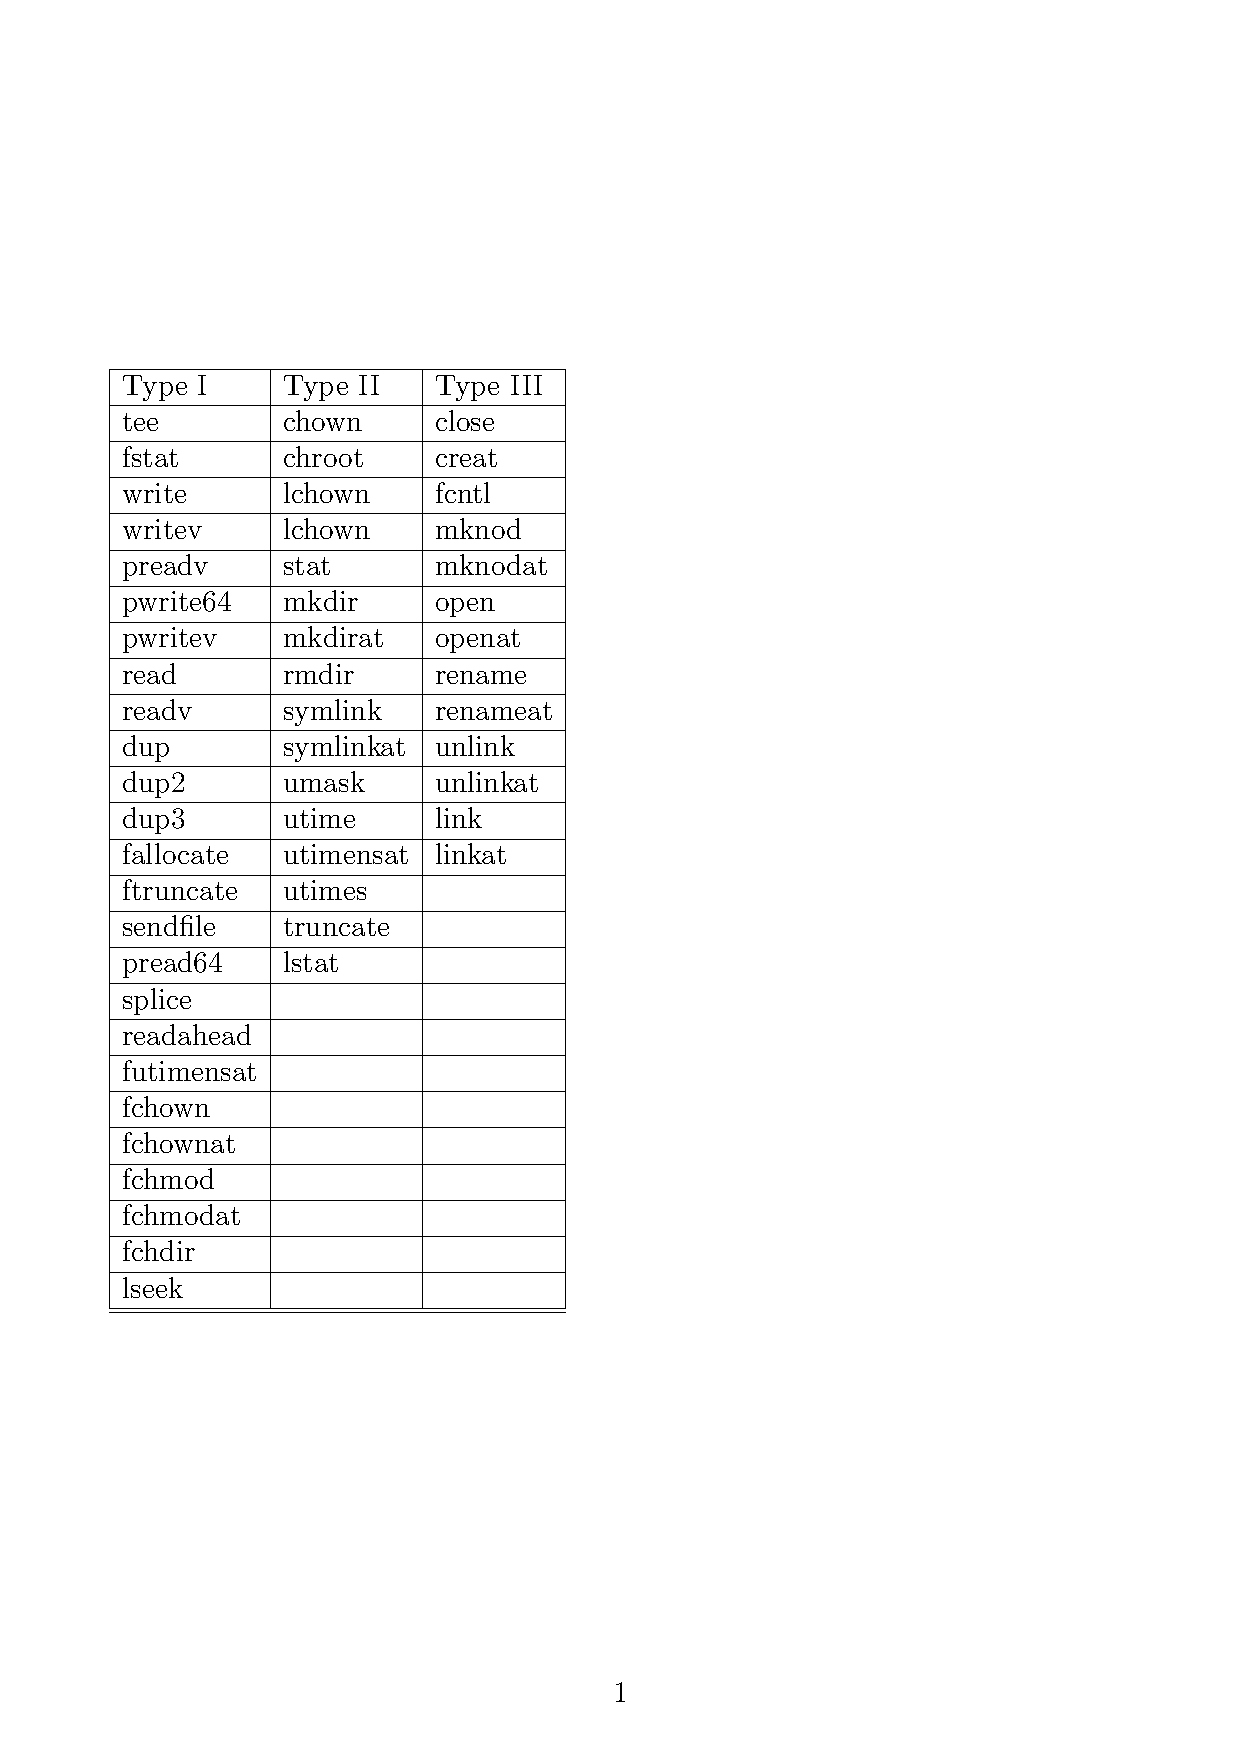
\includegraphics[width=1.0\columnwidth]{SysCalls}
  \caption{System call types}
  \label{fig:syscalltypes}
\end{figure}

We have identified a set of system calls that have to be mapped to PVM semantics.
These system calls belong to three types, as shown in ~\ref{fig:syscalltypes}

Type I, system calls that no not cause nodes in the graph to version.

Type II, system calls that act directly on paths and not via file handles.
PVM models type II system calls using the ephemeral local object $\phi$ as follows:

$$get(\phi)$$
$$get(\phi, eqv(g))$$
$$drop(\phi, eqv(g))$$
$$drop(\phi)$$

Type III, special case system calls that have to be defined individually.
Some type III system call mappings are shown below:

\texttt{Open} take a file path and returns a file descriptor.
This operation is mapped in OPUS as,

$$l = open(g):$$
$$get(l)$$
$$get(l, eqv(g))$$

\texttt{Close} takes a file descriptor as argument and releases the underlying resource.
This operation is mapped in OPUS as,

$$close(l):$$
$$drop(l, globals(l))$$
$$drop(l)$$

\texttt{Unlink} takes a file path as argument and deletes the file from the filesystem.
This is is mapped in OPUS as,

$$unlink(g):$$
$$get(\phi)$$
$$get(\phi,eqv(g))$$
$$\forall r.r \in locals(g).r\neq\phi.untie(r,g)$$
$$drop(\phi,eqv(g))$$
$$erem(eqv(g),g)$$
$$drop(\phi)$$

\texttt{Link} takes two file names as arguments and links the file path in the second argument as an alias of the file path in the first argument.
The PVM to Posix mapping for this system call is as follows,

$$link(a,b):$$
$$get(\phi)$$
$$get(\phi,eqv(a))$$
$$get(\phi,b)$$
$$eadd(eqv(a),b)$$
$$\forall r.a \in globals(r).r\neq\phi.tie(r,b)$$
$$drop(\phi,eqv(a))$$
$$drop(\phi)$$

\texttt{Rename} takes two files as argument, renaming the first file to the second.
This is a compound operation and can be defined in terms of other system calls as follows,

$$rename(a,b):$$
$$unlink(b)$$
$$link(a,b)$$
$$unlink(a)$$

In addition to the mappings defined above, the analyser also defines similar mappings for a number of other system calls.
Defining each mapping is beyond the scope of this document.

\section{Performance Evaluation}
In this section we evaluate the overheads of OPUS on scientific activities and workloads.
Our scope is limited to the most common types of scientific user activities, namely, 
package installation, file editing, code compilation, file archival/extraction, workloads requiring a runtime and finally compute intensive applications.
Representative workloads are chosen for each of these categories.

Two aspects of the system are of interest:
\begin{enumerate}
\item Temporal overheads introduced by the provenance capture and analysis components on end user applications.
\item Spatial overheads (memory and disk space) of processing and storing provenance data.
\end{enumerate}

To evaluate the temporal overheads we first setup a baseline for each workload with OPUS disabled.
We then enable OPUS and run the same set of workloads in the OPUS enabled environment.

OPUS has a number of configuration options for both the frontend and backend.
The frontend can be configured to run in two modes:
\begin{enumerate}
\item Full capture, where all events for which interposition is available are captured.
\item Lite capture, where certain events (e.g. reads and writes) are discarded.
\end{enumerate}

Similarly, the backend analyser can be configured to run in,
\begin{enumerate}
\item Logging mode, where the analyser does minimum processing on the system call data and logs it to disk.
\item PVM mode, where PVM operations are applied on each event received and a DAG is constructed.
\end{enumerate}

OPUS is evaluated with various combinations of configuration options for both the frontend and backend.
Each experiment is repeated ten times to account for variances in runtime due to system effects that we do not control.

\subsection{Workloads}
% TODO: Change the use of we here
We evaluate the overheads of OPUS using seven applications that are representative of workloads for a scientific user.

\paragraph{Package Installation:} apt-get is a commonly used package installation tool used in Unbuntu platforms and represents an I/O heavy workload.
We execute apt-get to install and remove the GNU Scientific Library (GSL) and measure the overheads when using OPUS.

\paragraph{File Editing:} Here we measure the overhead a developer experiences when editing a source code file.
To ensure that these measurements are accurate we use vimscript to automate the process of opening and editing a file.
This type of workload is both I/O and memory heavy and should be a reasonable test for the overheads imposed by OPUS.

\paragraph{Code Compilation:} Compilation is a very common activity that most scientific users perform.
To ensure we have a sufficiently complex code base to evaluate, we compile the linux kernl source code.
This activity produces a significant amount of I/O and process creation events which is captured by OPUS. 

\paragraph{File archival:} We use the tar and gzip programs on linux to evaluate the overheads of achival activity.
We tar and compress the linux kernel source tree to ensure a significant number of files are archived.

\paragraph{BLAST:} Blast represents a biological workload used to find protein sequences for a given species against a protein sequences database.
This represents a compute heavy workload.
% NOTE: ftp://ftp.ncbi.nih.gov/blast/executables/LATEST

\paragraph{Linpack:} is a program that solves a dense NxN system of linear equations Ax=b as it is a common problem in engineering and scientific computing.
Linpack uses the BLAS (Basic Linear Algebra Library) to perform matrix and vector operations.
This represents a compute heavy workload.
% https://github.com/2000nickels/linpackc

\paragraph{Python:} There is an increase in use of languages like python for scientific computing.
Python is an interpreted language and the runtime can perform several activities that are system or library call intensive.
Given the provenance capture mechanism OPUS uses, it is useful to understand the impact of the mechanism on such environments.
We run a sample python program from the BioPython package to measure the overheads imposed.

\todo{To be completed with graphs for each application}

Our evaluation is performed on an Intel i7-6820Hq CPU at 2.70GHz with 32 GB RAM, running Ubuntu 14.04 with a Linux 4.4.0 kernel.
We run each type of workload first with OPUS disabled to setup a baseline.
We then run all workloads with various configuration options for the frontend (Full or Light capture) and backend (Logging or PVM mode).

% TODO:



%We run our benchmarks with the various configurations of OPUS frontend and backend.
%The following combinations of configurations have been used:
%\begin{itemize}
%\item Full capture plus logging mode
%\item Lite capture plus logging mode
%\item Full capture plus PVM mode
%\item Lite capture plus PVM mode
%\end{itemize}


% We measure the overheads under various configurations for both the OPUS frontend and backend.
% i.e. full-fat and lite modes, backend in logging mode and PVM mode.
% Use of embedded vs standalone database.

% Application list:
% Code Compilation: Kernel Compile. Compilation of CBLAS, LAPACK, FFTW, LAPACK++.
% Package Installation: Use of apt-get and pip to install packages.
% Version Control: Git.
% File I/O: Postmark
% Archiving/Extracting: tar and untar
% Application Execution: BioPerl and BioPython, BLAST

% Discussion on what is the cause of the overheads on each of these workloads.
% Too many file matadata updates?
% Too many process and thread creations?
% Low overheads coz its CPU intensive? What meaningful provenance is recorded?
% Effect of analysis running on the same machine?
% Categorize syscalls. Which get called a lot, for what type of workload.
% Time breakdown by syscall.

% NOTES: How was PASS, CDE, Burrito evaluated?
% PASS and PA-NFS: linux compile, Postmark, Mercurial, BLAST
% CDE:
% BURRITO: 


%\begin{itemize}
%\item Temporal overheads of using OPUS. (Interposition overheads)
%\item Pathological case, \texttt{man} command. Single char reads and writes. (should this be in implementation?)
%\item Optimisations performed, aggregation, OPUS Lite etc. (implementation?)
%\item Performance evaluation of the analyser backend. Cost of DB operations.
%\item Spatial overheads: Average space used to store provenance, for scientific workloads.
%\item Comparing Neo4J with SQLite?
%\item https://docs.google.com/spreadsheets/d/13QqrShPEgjC91RKLnzcIfuliM-mZovhjO2vRkewWyJ0/edit?usp=sharing
%\item Look at how CDE was evaluated. SPEC, Real-World benchmarks.
%\end{itemize}

\section{Tools for Scientific Workloads}
\todo{To be expanded. Add screenshots of each tool output.}
\begin{itemize}
\item Debugging context changes. Detect changes in environment, command line params, library versions linked etc.
\item Show the command and output snapshot.
\item Tracking Computations. Capture scientific workflow from ad-hoc steps. Tools to visualise and scriptise the workflow.
\item Show the provenance graph figure here.
\item Archiving for compliance. EPSRC mandate to provide code and data used to produce results. Workflow archive tool, enables scientists to archive and upload their code and data used in experiments.
\item Post-hoc workflow construction
% NOTE: Maybe merge workflow tracking and archiving into one tool?
\end{itemize}


\section{Beyond Scientific Computing}
% TODO: Complete this
\begin{itemize}
\item OPUS as a provenance system can be used beyond the use-case of scientific computing.
\item The OPUS backend can consume data from any system call level tracing producer.
\item We have ported OPUS to work with data generated from DTrace instrumentation on FreeBSD.
\item This is in the context of the CADETS project. Explain CADETS briefly here.
\item OPUS will be one of the consumers of CADETS trace data and will generate provenance graph.
\item OPUS will run on the network and store data for higher level analysis.
\end{itemize}


\chapter{Trustworthy Capture of I/O}

In the previous chapter, we assumed provenance is captured in a trusted environment.
The trusted computing base (TCB) consisted of all software (user-space and kernel) and hardware on which applications executed.
In this chapter we explore the problem of capturing provenance in untrusted environments and discuss a new primitive, NORAD that enables capture of provenance for an application's I/O activities in a trustworthy and verifiable manner while maintaining a small TCB.

\section{Motivation}

For provenance to be useful it must be trustable.
In the past, provenance systems have assumed that a large part of the environment where they execute is trusted.
This ties the trustworthiness of provenance strongly with security of its environment which consists of the entire system software stack (OS and Hypervisor) and hardware (CPU, devices etc.).
A malicious insider or adversary could exploit vulnerabilities in this large software/hardware stack to either circumvent the provenance capture mechanism, resulting in incomplete provenance or falsify provenance data, destroying its integrity.
This renders the provenance unreliable and untrustworthy.

Ensuring trustworthiness of provenance is challenging.
We essentially need to ensure the following properties:
\begin{itemize}

\item \texttt{Completeness}: All relevant actions (provenance) pertaining to a unit of data (e.g. file, record, block, packet etc.) or computation (process, thread etc.) are captured.
There is no way to circumvent the provenance capture mechanism in order to make progress.

\item \texttt{Integrity}: The actions that represents the provenance cannot be modified or tampered with, either in flight or at rest. If the provenance is tampered with, one should be able to detect it and take appropriate action.

\item \texttt{Non-repudiation}: If the provenance records describe a set of actions in the past, one cannot deny those actions as not having taken place. Similarly, one cannot claim an action to have taken place if the provenance does not contain that information. That is, there is a strong tie between what the provenance describes as having happened and what actually happened on the underlying system. Completeness and integrity are necessary conditions for non-repudiation.

\end{itemize}


\subsection{Need for trustworthy verifiable provenance}
Once trustworthy and verifiable provenance is available, it has applications in a number of domains:

\begin{itemize}

\item \textbf{Legal:}
Use of electronic information such as emails, chats, documents etc. is admissable as evidence in legal proceedings.
However, one can always question the authenticity of such electronic information making it unusable in court.
Provenance can be used as proof to assert the authenticity of such electronic information.
However, unless the provenance is itself captured and stored in a trustworthy manner, it cannot be treated as reliable proof of the authenticity of electronic data.

\item \textbf{Regulatory Compliance:}
Healthcare Portability and Accountability act (HIPAA) ~\cite{HIPAA} requires logging of data accesses and modifications to medical records.
Similar efforts are happening in the UK's NHS system ~\cite{deepmind}, where all interaction with patient data are to be logged in a verifiable and trustworthy manner.
Other sectors such as finance also have such compliance requirements, for e.g. the Sarbanes-Oxley, Gramm-Leach-Bliley and the UK's Data Protection act require proper documentation and audit trails for financial records.
These audit trails provide a form of provenance in the financial industry.
Unless these audit trails are trustworthy and verifiable they cannot be used as proof for an activity or transaction.

\item \textbf{Scientific Computing:}
Scientific computing has for a long time advocated the capture of provenance into its data generation, workflows and processing.
Over the years several projects ~\cite{PASS, SPADE, OPUS} have integrated provenance capture at the system's level to aid such activity.
Once provenance is available it enables us to verify the authenticity and quality of a given result.
However, if the provenance itself can be forged or tampered with then the provenance can be asserted as proof for any desired output. 
Unless provenance is trustworhty and verifiable, its use as proof in the context of scientific computing becomes meaningless.

\item \textbf{Computer Security:}
Provenance has applications in computer systems security.
Provenance essentially captures interactions between computational processes, flow of information between these processes and the context in which all this happens.
When done at the system level, it allows us to build powerful security tools to investigate or monitor activities such as intrusions and data exfiltration either retroactively or in real-time.
However, if the provenance capture mechanism can be compromised or the provenance data falsified there is no guarantee that these tools will be effective.

\end{itemize}

\section{The Challenges of Trustworthy Provenance Capture}

In the past trustworthy capture of provenance has often meant ensuring security of provenance data at rest.
The most notable work on this is SPROV ~\cite{sprov} which uses the concept of provenance chains to ensure integrity and confidentiality of provenance records.
However, merely providing confidentiality and integrity of provenance records at rest does not guarantee that the provenance is trustworthy.
We also require the mechanism that does the provenance capture to be complete, tamper-resistant and verifiable.

Patric McDaniel et al. ~\cite{patric} discuss the design principles of such a secure provenance capture mechanism based on the well-known concept of a reference monitor ~\cite{refmon} .
A reference monitor enforces an access control policy over user operations on the system while ensuring that it is non-bypassable, tamper proof, always invoked and evaluable.

In the traditional application-OS system design the OS plays the role of a reference monitor as all application activities relating to device I/O and process creation/destruction have to be mediated via the OS.
Whole-system provenance projects such as ~\cite{AdamBates, CamFlow} therefore implement provenance capture in the OS leveraging the linux security modules ~\cite{LSMFramework} framework.
However, most mainstream OS implementations are complex comprising of hundreds of thousands of lines of code, often implemented using low-level unsafe languages.
Even a single vulnerability in this code base could be exploited by attackers, potentially leading to a privilege esclation and ultimately a compromise of the provenance capture mechanism.
Ensuring that such complex systems are bug free or verifying their correctness properties is not trivial.

Recent advances as Intel SGX and ARM Trustzone offer some hope as they provide hardware support for trusted execution.
Intel SGX is especially of interest since it offers mechanisms to preserve the integrity and confidentiality of code and data without requiring to trust other privileged layers such as the OS, hypervisor, firmware or SMM code.
Depriviliging parts of the OS to run in such trusted computing environments can allow us to capture provenance in a trustworthy manner.

Our design, discussed in the next section uses this insight and offers a new primitive for capturing provenance in a trustworthy and verifiable manner by leveraging Intel SGX for trusted execution.
To show a proof-of-concept system, we focus on capturing I/O events in a trustworthy manner as I/O activity information constitutes a major part of data provenance.


\section{NORAD}

Most applications have some necessity to perform I/O, for example to read configuration files, write output logs, store database records, access storage across the network etc.
Capturing these I/O activities in a system allows us to build provenance of data.
Data provenance solutions in the past ~\cite{PASS, StoryBook} have used mechanisms where I/O activities in a system are interposed and captured to retrospectively build a provenance graph.
However, most of these solutions implement their capture component in the OS and require trusting the entire OS stack.
In this section we present a new primitive that allows the trustworthy capture of I/O in a system without having to trust the underlying OS and higher privileged software.
%We first describe a general design that is applicable for both disk and network I/O, along with an informal proof of correctness followed by an implementation and evaluation for disk I/O.

\subsection{Software Guard Extensions (SGX) Overview}
Our design for trustworthy capture of I/O leverages Intel SGX for trusted execution of applications.
Therefore we provide a brief overview of SGX to aid understanding of this work.

SGX (Software Guard Extensions) has been commercially available since 2015 as part of Intel’s Skylake series of processors.
SGX enables an application to create an inverse sandbox wherein a portion of application memory, called an enclave is protected from the rest of the system, including the OS, hypervisor and SMM software.
Enclave memory is also protected from direct access by peripheral devices.
SGX hardware guarantees the confidentiality and integrity of the contents (code and data) of the enclave.

SGX enclaves are provisioned and initialised by the untrusted OS in Ring-0.
While loading the enclave its contents are cryptographically hashed by the CPU.
The final hash value after initialisation becomes the measurement of the enclave which can be used for attestation.
The attestation mechanism provides proof to either a local or remote party that the enclave has a specific measurement hash and that it is executing on a genuine SGX enabled CPU.

Once an enclave has been initialised applications can enter and execute enclave code via a special instruction EENTER.
A major limitation of SGX, however, is that enclave code can only be executed in ring-3 or user-mode.
Another fundamental limitation of SGX is that instructions such as \texttt{SYSCALL} are disallowed inside enclaves since it results in a privilege switch to ring-0 mode.
In order to access system services applications must first exit their enclave before invoking system calls.
Therefore, without significant effort to port system code to run within enclaves ~\cite{haeven}, we cannot guarantee the security and trustworthiness of system services.
As we shall see in the sections below, our design addresses this problem and enables trustworthy capture of I/O without requiring the whole OS to run within SGX.

\subsection{Threat Model}
We consider a powerful adversary that controls the entire software stack on a server except trusted code that runs within SGX enclaves.
The adversary could be an untrusted administrator, a user who has gained root privileges or an outside attacker who has exploited a vulnerability to compromise the OS.
The goals of the adversary are as follows:
\begin{itemize}
\item Perform I/O to either read, modify, delete existing data in storage.
\item Interpose I/O from other users to subvert their requests/data.
\item Record requests in flight from genuine users and replay them at a later point in time to corrupt or rollback data in storage.
\item Carry out these attacks stealthly by being undetectable to any OS level auditing or provenance tracking mechanism.
\item Achieve stealth by attacking the provenance capture mechanim itself leading to circumvention or falsification of provenance.
\end{itemize}


Since the adversary controls all layers in the software stack, denial-of-service attacks wherein I/O requests are discarded or genuine trusted applications are not scheduled at all for execution is possible.
Our design for I/O does not explicitly address such an attack by preventing it, instead, it ensures that even the attacker cannot perform I/O and make forward progress without being detected.
Similarly, side-channel attacks ~\cite{sideat1, sideat2} are not addressed by our design.
Side-channel attacks on trusted hardware is an active area of research ~\cite{sidemiti1, sidemiti2} and building side-channel defense mechanisms for I/O is a future exercise.
Our design also does not explicitly address the problem of ensuring confidentiality of data or its provenance as this can be solved by using encryption.

~\paragraph{Trusted Computing Base (TCB):}
Our TCB consists of the SGX enabled CPU, a trusted I/O device (storage disk or network card) and all code that runs inside SGX enclaves.
Enclave code is signed and provided by a trusted third party (for example an authorised group of auditors).
Similarly, the trusted I/O device with a thin firmware interposition layer is also provided by the trusted third party.

We assume that the attacker cannot perform physical attacks on the CPU by opening the processor package to extract secrets or corrupt its internal state.
Similarly, we assume that the trusted I/O device cannot be reflashed or physically attacked by the adversary.

\subsection{Requirements for Trustworthy Capture of I/O}

Given the threat model in ~\ref{sec:threatmodel} we attempt to answer the question "What are the requirements for trustworthy capture of I/O?".

We've identified three key requirements to provide this support:

\begin{enumerate}

\item \texttt{Capture across layers of abstractions:}
The OS presents applications with an abstracted view of I/O devices and the low-level interface required to interact with these devices.
For example, in case of disk I/O, the disk hardware is presented as a block device where data in chunks of blocks (typically 4K per block) can be stored and retrieved.
These chunks of blocks are in turn grouped and identified via the inode datastructure in the OS's filesystem.
However, the view that an application has is that of a simple filename path and uses stream operations to read and write data to the file.
Similarly, for network I/O the OS abstracts away the process of sending and receiving network packets.
Most applications only send and receive data streams to a specific IP address and port tuple.
Merely capturing events at the level of abstraction that an application observes is not sufficient.
We must also capture the underlying OS-level events pertaining to the application's request in a trustworthy manner.

\item \texttt{Capture must be tamper-proof and non-bypassable:}
If we implement a mechanism that captures application I/O requests and its corresponding low-level actions in the OS there is no guarantee that capture is trustworthy.
An adversary that controls the OS could attack the capture system itself, destroying its integrity.
Any capture performed thereafter will be unreliable.
Even if the capture components themselves are secure and tamper-proof an attacker that controls the OS could easily circumvent/bypass them by accessing hardware devices directly or by modifying in-flight requests to hardware post-capture.
To mitigate against such attacks the OS should be restricted to only carry out low-level actions approved and recorded by a tamper-proof monitor.
This leads to the requirement for a non-forgeable capability based mechanism.

\item \texttt{Verification by Trusted devices:}
Once the OS obtains a capability to perform a certain low-level action on an I/O device, it can then access the underlying I/O device hardware to fulfill that request.
However, if the I/O device does not verify the actions of the OS, once again there is no guarantee that the OS fullfilled that request failthfully.
A compromised OS could (i) throw away application requests, leading to data loss or
(ii) modify requests at the device-driver level, leading to subversion of data or
(iii) fabricate data as having originated from a valid hardware device.

To mitigate against such attacks, a trusted end-point device is necessary to verify and acknowledge (the success or failure) the OS's request against the non-forgeable capability that it provides.

\end{enumerate}


\subsection{NORAD Access Control} 

To satisfy the requirements described in ~\ref{sec:requirements} we need a reference validation mechanism that enforces an access control policy for I/O.
To this end we introduce a new primitive for I/O, NORAD access control.

\subsubsection{Design Principles} 
Our design for NORAD access control is based on the following key principles.

\begin{enumerate}
\item \textbf{Secure Capture of I/O.}
When a user-space application makes a system call, for example to write a file to disk or to send a stream of data over the network, we must capture this event.
To ensure that the capture is performed in a secure trusted environment, the system call capture code executes inside an SGX enclave.
The system call capture component can be impemented as an I/O library that applications can link against or as an interposition layer that is seamless to applications.

In addition to the system call capture, we also require a mechanism to capture the low-level actions that the OS performs securely to service the system call.
To achieve this, we introduce the concept of an \texttt{Arbiter}.
The \texttt{Ariter} is a non-forgeable, non-bypassable, evaluable user-space process that executes inside an SGX enclave.
The security properties provided by SGX ensures the integrity, confidentiality and freshness of the contents (code and data) of the Arbiter.
The low-level operations pertaining to a I/O related system call are captured by the Arbiter.
In case of disk I/O, the Arbiter captures the block-level reads and writes as the untrusted OS is forced to provide this information in order to make forward progress.
Similarly, for network I/O the Arbiter captures details about individual packets as the OS sends or receives packets to/from the network device.

However, this implies that we trust the underlying OS to perform the correct low-level operation.
A compromised OS may not necessarily perform the right low-level operation pertaining to a system call request.
To understand this point, lets take the example of file I/O.
When a file is opened and read by an application, an in-kernel filesystem fetches the right sets of blocks representing the file's data from storage.
This is possible since the file system maintains the metadata (inodes, directory entry etc.) that maps the file to its block-level representation on the storage device.
In a compromised OS there is no guarantee that this metadata is correctly maintained.
Therefore, even if we faithfully record the low-level operation, in this case of the file system, the recorded information may not be useful.
To reason about what happened to data on the storage device we require internal knowledge of the semantics (file to blocks mapping for example) of the file system.

In our design we address this problem, by moving critical parts of the OS to run within the Arbiter while still ensuring that the Arbiter is reasonably small and evaluable.
In case of the file I/O, we can implement a simple block-based file system that runs entirely inside the Arbiter using existing user-space file system frameworks such as FUSE ~\cite{FUSE}.
This ensures that I/O operations across layers of abstractions are captured in a trustworthy manner.

\item \textbf{Token Generation.}
The Arbiter is a user-space process, therefore interfacing with I/O hardware directly is a challenge.
Barring special cases ~\cite{kernelbypass, inteldpdk}, access to hardware still requires mediation via the OS.
The device drivers managed by the OS interface with hardware devices to perform the relevant operations.
Therefore, a compromised OS could still tamper with the low-level operation parameters, causing the captured I/O information to differ from the actual I/O activity.

To mitigate against such attacks the Arbiter generates a non-forgeable \texttt{token} (or capability) and hands it to the OS.
The OS is then forced to use this \texttt{token} in order to make forward progress.
Tokens for low-level operations can be generated using cryptographic primitives such as Message Authentication Codes (MAC) or Digital Signatures ~\cite{MAC, DigitalSig}.

The OS cannot proceed to perform the required I/O operation without acquiring this token.

\item \textbf{Device-level Verification.}
To ensure that the OS only requests for the device-level operation that is approved by the Arbiter, we require a I/O device to verify the intentions of the OS.
The I/O device used as part of NORAD access control therefore has a thin modified firmware layer which checks the authenticity, integrity and freshness of the device-level request against the token provided.
The device can in turn generate an acknowledgement which can be handed back to the application confirming the success/failure of the I/O operation.

\end{enumerate}

\subsubsection{Access Control Protocol}
Combining the three design principles in ~\ref{sec:designprinciples}, we now describe the NORAD access control protocol using disk I/O as an example.

First, we define the terminologies used in the protocol.
Then, we briefly describe the various entities involved in I/O before proceeding to explain the protocol with the help of figures ~\ref{fig:noradhld} and ~\ref{fig:noradproto}.

\paragraph{Terminologies:}
\begin{itemize}
\item \underline{Key:} A secret symmetric key shared between two trusted entities.
\item \underline{MAC:} A cryptographic primitive used to check the authenticity and integrity of messages.
\item \underline{Nonce:} A unique integer value provided as part of a message to ensure freshness of the message.
\item \underline{Enclave:} A secure region of memory whose integrity, confidentiality and freshness is protected by Intel SGX hardware.
\end{itemize}

\paragraph{Entities:}
The NORAD access control protocol for I/O primarily inolves communication between four key entities in the system.
\begin{itemize}
\item \textbf{Application:} User-space processes performing I/O on the trusted storage device.
The application invokes system calls to the untrusted OS to access data on the trusted storage device.

\item \textbf{Untrusted OS:} The untrusted OS executes with ring-0 privileges, manages hardware device and services applications requests.

\item \textbf{Arbiter:} A process executing with ring-3 privileges.
The Arbiter implements a simple block-based filesystem and captures the block-level I/O requests to the trusted storage device.
It also generates a non-forgeable \texttt{token} for each block-level operation performed by the OS.

\item \textbf{Trusted Storage:} A storage device containing firmware functionality to verify OS provided block-level requests against the Arbiter generated token.

\end{itemize}


\begin{figure}[t!]
  \centering
    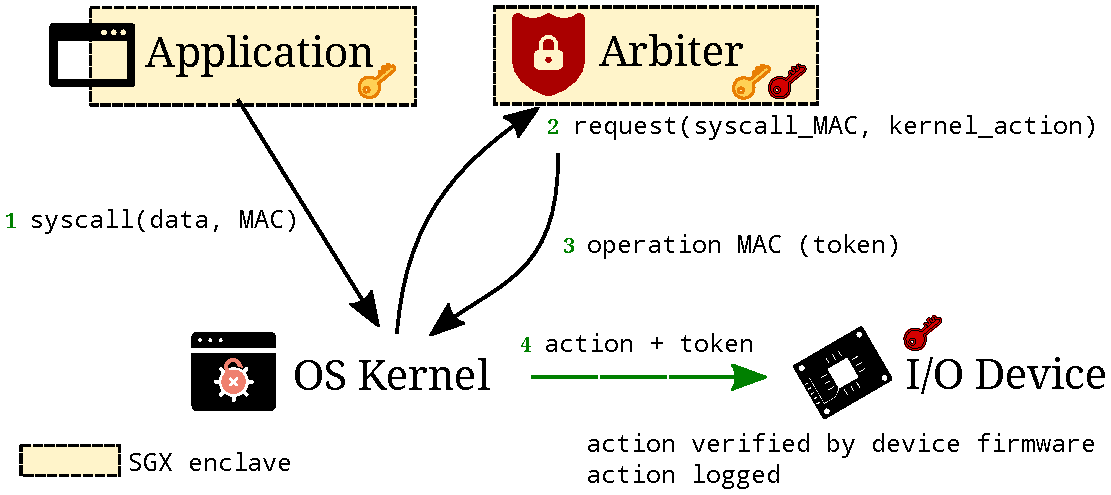
\includegraphics[width=1.0\columnwidth]{noradhld}
  \caption{NORAD I/O}
  \label{fig:noradhld}
\end{figure}

\paragraph{Bootstrap and Setup:}
We boot an uncompromised signed kernel image.
The system is initially disconnected from the network.
A trusted storage device, provided by authorised auditors, is initialised by the kernel as part of the boot process.

The trusted storage contains two partitions,
(i) to store user and application data and
(ii) to store system call and block level request data as provenance.
The trusted storage device also contains a modified firmware layer and a secret key $K_D$.

The auditors also provide 
(i) a library $L_D$ that applications are required to link against to invoke disk I/O operations and
(ii) an executable for the Arbiter process implementing a block-based filesystem.
Both the library and the Arbiter are trusted and execute within an Intel SGX enclave.

The Arbiter binary is provisioned with the same key $K_D$ as that of the trusted storage device.
This provisioning is performed by the trusted auditors when the binary for the Arbiter is compiled.
The confidentiality of the key $K_D$ is ensured by encrypting the key using SGX's sealing ~\cite{sgxsealing} functionality.
Only enclaves with the auditor's signing identity (based on MRSIGNER ~\cite{mrsigner} value) can unseal the key.

The trusted storage device and the Arbiter also initialise a nonce $N_D$.
The nonce enables both the Arbiter and the trusted storage to check the freshness of messages exchanged via the untrusted OS.
The simplest scheme is to initialise the $N_D$ to zero during boot.
$N_D$ is incremented in lock-step by both the Arbiter and the trusted storage device for each request/response message.

When the Arbiter process is started it mounts the filesystem from trusted storage by reading its superblock information.
The process of reading the superblock uses the same access control protocol discussed in ~\ref{sec:diskioflow}.

In order to ensure that all requests reach the Arbiter, caching (buffer cache, inode cache etc.) at the virtual file system layer (VFS) are disabled.
Instead, these caches are maintained by the filesystem implemented inside the Arbiter.

Once this setup is complete the system can be connected to the network and users can begin executing their applications.
After this point the OS is potentially vulnerable to attacks.

\todo{Redo image according to the description}

\paragraph{Loading Applications:}
Applications requiring access to trusted storage link against the library $L_D$ to invoke I/O operations.
As shown in figure ~\ref{fig:noradhld}, the library executes as part of the application's address space but within an SGX enclave.
When an initialisation routine is invoked, the library $L_D$ requests a key $K_A$ and an application specific nonce $N_A$ from the Arbiter process.
This is done via a shared memory region that the application shares with the Arbiter, refer figure ~\ref{fig:noradhld}.
To ensure confidentiality of key $K_A$, the Arbiter seals the key using SGXs sealing functionality before writing it to shared memory.
The library $L_D$ can unseal this key inside the enclave.
The nonce $N_A$ is incremented by both the application and the Arbiter in lock-step as each system call is invoked via the library $L_D$.
This ensures checking the freshness of system call information captured by the trusted library $L_D$.

\subsubsection{Disk I/O Flow:}

\begin{figure}[t!]
  \centering
    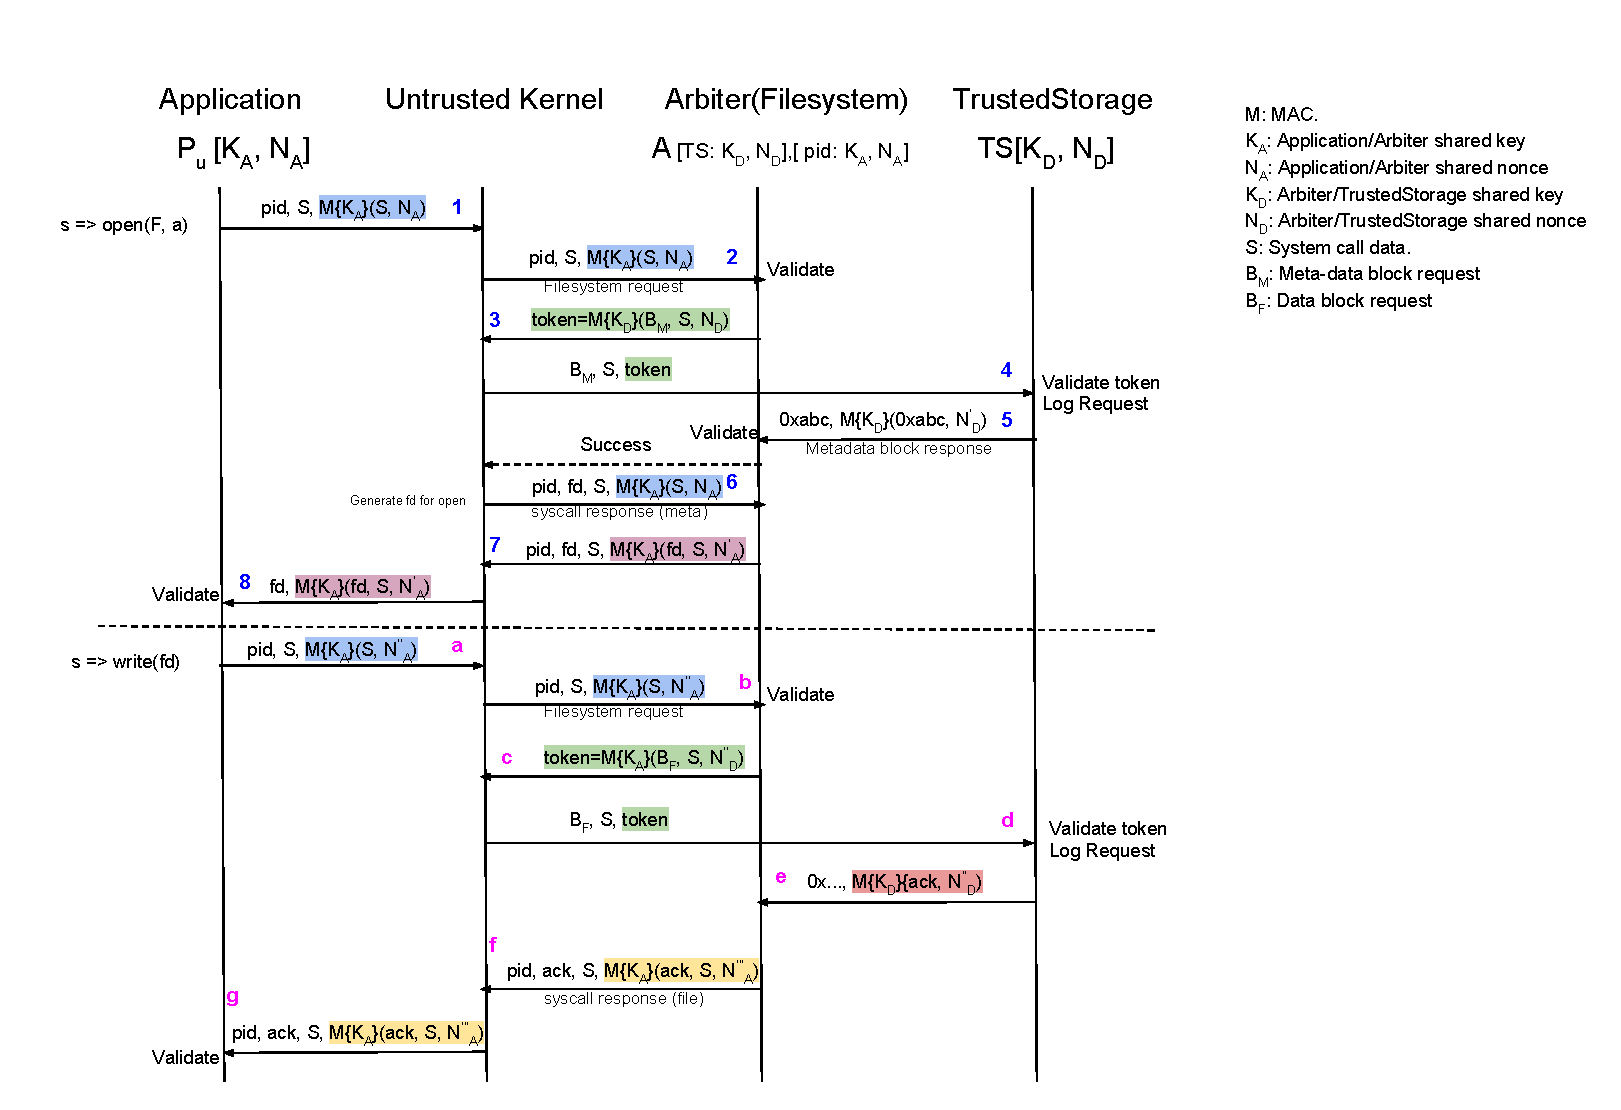
\includegraphics[width=1.0\columnwidth]{norad_access_control}
  \caption{NORAD access control protocol}
  \label{fig:noradproto}
\end{figure}

To understand how a file I/O request and response works let us look at an example of a process that opens a file and writes data to it.
We assume that the file is opened with the \texttt{SYNC} flag as this ensures that the data is physically written to the underlying storage device before the application can proceed further.
The steps in the protocol for each of these operations is illustrated in figure ~\ref{fig:noradproto}.

% File open for writing example
The steps 1-8 shown in figure ~\ref{fig:noradproto} explains the steps when the \texttt{open} system call is called on file \texttt{F}.
File \texttt{F} is stored on the primary partition in the trusted storage device.

\begin{enumerate}[Step 1:]

\item When an application invokes the \texttt{open} system call, the syscall data consisting of file name, flags and mode are captured by the trusted library $L_D$.
The library also generates a MAC of the syscall data using key $K_A$ and nonce $N_A$.
The syscall request along with its identity (e.g. pid) and MAC is passed to the kernel.

\item The syscall is serviced via the VFS in the untrusted kernel. The VFS forwards the request to the Arbiter (file system) process along with its MAC.

\item The Arbiter validates the request from VFS (syscall request) against its MAC using key $K_A$ and nonce $N_A$ and if successful forwards the request to the file system executing as part of its address space.
If the file system does not contain the file meta-data in its cache, it initiates a request to read meta-data blocks, $B_M$ from trusted storage.
The Arbiter generates a \texttt{token} (MAC) for block request $B_M$ along with its corresponding syscall data $S$ using key $K_D$ and nonce $N_D$.
The request data and token are provided to the kernel.

\item The block layer in the kernel forwards the Arbiter provided request and token to the trusted storage device via the appropriate device driver.

\item The storage device validates the request data against the token provided by the kernel.
If successful, the appropriate blocks are fetched and returned back as response to the Arbiter via the kernel along with a MAC of the response using key $K_D$ and an incremented nonce value $N^\prime_D$.
The request (block and syscall information) is logged as provenance in a seperate internal partition that the kernel cannot write to.

\item Once the Arbiter (filesystem) validates the response from the trusted storage, the kernel generates a file descriptor (fd) as a response for the \texttt{open} syscall.
This information is again provided to the Arbiter for attestation.

\item The Arbiter ties the \texttt{fd} to the \texttt{open} syscall request and generates a MAC using key $K_A$ and incremented nonce $N^\prime_A$.  

\item The kernel returns the \texttt{fd} back to the application along with the Arbiter provided MAC as proof that the \texttt{fd} was generated for valid file meta-data.
This is validated by the library $L_D$ using key $K_A$ and nonce $N^\prime_A$.

\end{enumerate}

Once the application receives a filed descriptor, it can begin writing data to the device using it as a reference.
Steps a-h describes request and response flow for writing data to trusted storage.

\begin{enumerate}[Step a:]

\item When the application invokes the \texttt{write} syscall on \texttt{fd} passing it a buffer, the trusted library $L_D$ captures the request information and generates a MAC on its contents using key $K_A$ and a new incremented nonce value $N^{\prime\prime}_A$.

\item The syscall $S$ is handled by VFS in the kernel and forwards the request to the Arbiter process along with its MAC.

\item The Arbiter validates the request against its MAC using key $K_A$ and nonce $N^{\prime\prime}_A$.
If successful, forwards the request to the filesystem component in its address space.
The file system issues a block write request $B_F$ to persist the data in trusted storage.
The Arbiter generates a \texttt{token} for request $B_F$, syscall $S$ using key $K_D$ and nonce $N^{\prime\prime}_D$.
This \texttt{token} is then passed to the kernel to service the block write request.

\item This block write request is then provided by the kernel to the trusted storage device.

\item The trusted storage firmware verfies the block request against its token.
If successful, the appropriate blocks on physical storage are written to and modified.
An acknowledgement message using key $K_D$ a new incremented nonce value $N^\prime\prime_D$ is passed to the kernel as response.
The request details are logged as provenance in the internal partition against the respective blocks.

\item The Arbiter validates the device acknowledgement against its token.

\item The acknowlewdgement is then tied to the corresponding syscall request made by the application.
A MAC of this information is generated using key $K_A$ and incrmented nonce $N\prime\prime\prime_A$.
This MAC is then passed to the kernel.

\item The kernel then relays this information back to the application, which validates the response against the MAC provided.

\end{enumerate}

\subsubsection{Security Properties:}
We now discuss some of the security guarantees provided by NORAD access control for disk I/O.

\begin{itemize}

\item \textbf{Non-Bypassability:}
All disk I/O to trusted storage must use the NORAD access control mechanism.
Direct access to trusted storage, bypassing the access control mechanism, will be detected and rejected by the trusted storage device.
This is guaranteed by the protocol since the trusted storage device verifies requests against a non-forgeable token (MAC).
Tokens can only be generated by a tamper-proof Arbiter that shares a secret key with the trusted storage device.
Non-bypassability provides us the assurance that the audit history for blocks and files (comprising of request details) is always captured.

\item \textbf{Tamper Detection:}
All application generated syscalls to the trusted storage are captured and a non-forgeable MAC of this syscall information is used to detect any tampering to the syscall information in-flight.
Similarly, the block-level events generated by the filesystem (Arbiter) are captured along with a MAC of the request data.
Again, any tampering of block-level requests can be detected.

\item \textbf{Data Loss Detection:}
The trusted storage provides an acknowledgement back to the Arbiter for each block-level request handled.
Therefore, in case of writes to trusted storage, an application can verify if its writes actually reached storage.
If a compromised OS throws away an application'w write request, it can be detected.

\item \textbf{Freshness:}
The MAC values generted in both the request and response paths use fresh nonce values.
Nonce values are incremented each time by the sender and receiver of a message (request or response).
This guarantees that a new MAC value is generated each time even if the rest of the data (MAC payload) remains the same.
Even if an attacker knows the nonce value for a message, generating the right MAC value for a request/request will require knowledge of a key which is a secret that only the sender and receiver share.

\end{itemize}

\subsubsection{Informal Proofs of Correctness}
\begin{itemize}
\item \texttt{Theorem 1:} Support R represents a request to access trusted storage, R must be accompanied by valid token T in order to make forward progress. 

\item \texttt{Theorem 2:} Suppose R represents an application request to access storage, any tampering with R can be detected.

\item \texttt{Theorem 3:} Suppose R is a request to access trusted storage, R is always a fresh request.

\todo{Complete these informal proofs}
\end {itemize}


\subsubsection{Challenges:}
The NORAD access control protocol poses a number of challenges on existing systems.
We discuss these challenges and possible solutions to them.

\begin{itemize}

\item \texttt{Increased Context Switches:}
The Arbiter implements a block-based filesystem that reads and writes data to a block-device.
Since the Arbiter runs in user-space, all file I/O to trusted storage adds extra context switches from kernel to user-space in both the request and response paths.
Added to this is the cost of switching in and out of SGX enclaves.
There are existing solutions that reduce the cost of switching in and out of SGX enclaves ~\cite{hotcalls, eleos}, however to mitigate the cost of switching between kernel and user context we need to implement a fast IPC mechanism (e.g. shared memory) for communication across privilege layers.

\item \texttt{Unreliable Identifiers:}
The I/O request data captured contains both the syscall as well as the underlying block-level request information.
In order to use this captured information to reason about I/O activity on the system, we require identifiers such as pid, process/binary name, uid, gid, etc.
However, the kernel provides these identifiers.
If the kernel is compromised these labels/identifiers become unreliable.
One solution to this problem could be to deprivilege parts of the kernel that generate these identifiers to execute within the trusted Arbiter.
However, moving more and more functionality into the Arbiter can make its code complex and prone to bugs, and introduce added runtime overheads.
These trade-off needs to be understood and evaluated.

\item \texttt{Dealing with Asynchrony and reordering of requests:}
In our design entities involved in file I/O increment nonce values after each request-response cycle either in lock-step.
However, this assumes that all I/O operations happen synchronously.
In reality most OS I/O schedulers reorder requests to the device and perform I/O asynchronously for performance reasons.
This breaks our initial assumption and can cause nonce values to go out of sync.
A solution to this problem is to maintain a sliding window of acceptable nonce values (window size could be based on the block device queue size) instead of just expecting a higher nonce value than previously seen.

\end{itemize}

\subsubsection{NORAD Access Control Prototype Implementation}
The prototype implementation of NORAD access control consists of a user-space library, NORADlib (approx. 1300 lines of C and C++ code) and a kernel module (approx. 700 lines of C).
There are no changes to existing kernel source code and drivers.
Application requiring trustworthy capture of I/O must use the NORADlib API.
The kernel module is implemented as a stackable block device driver that exposes a virtual device representing trusted storage.
The virtual device overlays an actual target physical device.

Since this is a proof-of-concept implementation, we emulate the firmware extension functionality to validate requests within the stackable block driver.
The firmware emulation code is small and lightweight layer that interposes existing device firmware's request handling functionality.

The prototype is only used to evaluate the performance overheads imposed by NORAD access control in the disk I/O path. 
To guarantee the security properties discussed in section~\ref{sec:secproperties} a storage device with an extensible firmware must be used.

\paragraph {Simiplification of the design:}
We simplify the design of NORAD access control by moving the functionality of the Arbiter into NORADlib.
NORADlib implements an API to access a raw block device and perform append only operations on blocks.
Filesystems and applications like databases read and write blocks directly, therefore this simplification to the design serves to evaluate such systems.

\paragraph {Using NORAD Access Control:}
When an application invokes the NORADlib API, it opens a virtual block device using the \texttt{O\_DIRECT} flag.
This provides the library raw access to the device to read/write blocks directly, bypassing the kernel VFS layer and any caching.
Caching of reads and buffering of writes is implemented within the library.
NORADlib runs inside an SGX enclave and is provisioned with a secret symmetric key shared with the trusted device and an initial nonce value.
The library uses Intel SGX SDK (version 1.7) internally to implement enclave functionality.
A high performance MAC algorithm, VMAC ~\cite{vmac} (ported to run inside SGX enclave) is used by the library to compute MACs (tokens) for block request and response messages.

For each block request, the library genertes a tokens and passes it to the underlying device driver (emulating the firmaware extension) via an \texttt{ioctl}.
The driver verfies each request by computing a MAC of the request contents and comparing against its corresponding token.
In the response path, the driver generates a similar token for the contens of the response which is read by the library using another \texttt{ioctl} and verified.

A performance evaluation of our prototype is discussed in ~\ref{sec:noradacceval}

\section{Applications of NORAD Access Control}

Once a primitive like NORAD access control is available, a number of use-cases are possible.
Take for example the logging of financial transactions in banks as part of a government mandate or storing system level activities in a cloud for regulatory compliance or logging of events from a distributed system to build provenance of data.
All these activities involves logging of data in a non-repudiable manner.
This kind of data logging is usually append only and has the property that it is immutable.
That is the data is only written once but read many times.
Traditionally WORM storage devices and servers provided this property of immutability, but only for data at rest.
NORAD access control on the other hand allows verification of the integrity of requests and data when they are in flight.
When combined with a secure trusted filesystem that implements WORM or COW (copy-on-write) semantics, NORAD access control can be used to implement such non-repudiable logging solutions where authenticity and integrity of data in-flight and at rest are guaranteed.

However, NORAD access control requires the use of a trusted storage device.
The trusted storage runs a modified firmware that verifies the authenticity and integrity of each device access request that the OS provides.
All data and audit information (request details) for each block is then stored on the trusted device.

The use of a trusted storage device to store all application data poses a major shortcoming.
A number of vendor specific device firmware code has to be understood and augmented to implement the functionality to validate requests.
Most firmware implementations are proprietary, with no access to their source code.
Therefore, scaling the design (of NORAD access control) to work with various vendor specific implementations is hard.
\texttt{Is there a way to reason about the trustworthiness of data without requiring the data to reside on trusted storage?}
We attempt to address this question in this section and discuss the design for a verifiable logging solution using NORAD access control.
This design is based on several key insights which we now discuss.


\subsection{Key Insights}

\begin{itemize}

\item NORAD access control provides the security properties of non-bypassability, tamper-detection, data-loss detection and freshness of requests ~\ref{sec:secproperties}.
Barring the property of non-bypassability the other three security properties essentially guarantee integrity of data.
This integrity check is however performed eagerly (during an I/O request/response flow) by the NORAD access control protocol.
Instead of detecting integrity violations eagerly when the I/O operation is in flight, detecting integerity violation lazily during a read operation is sufficient in most cases.

\item In order to detect integrity violations lazily, during reads, a cryptographic proof of the integrity of data blocks must be provided.
If this proof if provided by the untrusted OS, it can be verified by a secure trusted entity against a secure copy of the proof that it maintains.

\item The proof can be updated and maintained by the trusted entity in memory and persisted to trusted storage periodically.

\item The NORAD access control mechanism can be used to guarantee persistence of this proof in trusted storage.

\item The storage requirement for the proof itself is much lesser when compared to the actual data.
This enables us to store the proof on a small trusted device.

\end{itemize}

\subsection{Verifiable Logging}
We describe a mechanism for verfiable logging when both the OS and the data storage medium are untrusted using figure ~\ref{fig:verilog}.

\paragraph{Logging Service:}
Consider a logging service that accepts an encrypted stream of events from machines in a distributed system.
The job of of the logger is to receive the data and store it on disk so that it can be processed asynchronously by other applications.
Since the OS is untrusted, the integrity of the contents (code and data) of the logger must be protected.
We can ensure its integrity by running the logging service withing an SGX enclave.
A secure (TLS) connection to the logging service can be established from the outside to provide data to be logged.
Running the logger within an enclave and using TLS to receive data from the network ensures the integrity of the logger and the data it receives.
However, a compromised OS could still perform denial-of-service attacks by not scheduling the application at all or by not allowing the TLS connection to be established in the first place.
Addressing such types of attacks is beyond the scope of this discussion.

\paragraph{Storage Organisation:}
Unlike the NORAD access control mechanism, for verifiable logging we use an untrusted storage and a small amount of trusted storage.
The untrusted storage consists of two partitions,
(i) a data partition where the event streams are logged and
(ii) a partition to store a merkel tree as proof of integrity of each data block.
The size of each partition can be decided based on the amount of data required for storage.
For example, if the maximum size of the data partition is 1TB, with 4K as the maximum block size, we have over 268 million blocks.
If we use a 256 bit hash and a branching factor of 128 (since a 4K block would then hold 128 hashes), we would require less than 10GB of space to store the merkel tree.

The trusted storage can be any device such as a TPM chip or a removable USB stick with a firmware interposition layer to implement the verification required for NORAD access control protocol.
The trusted device only stores the merkel root, a secret key and nonce value and requires very little capacity.
The secret key and nonce are shared with an Arbiter type mechanism as described in the NORAD access control protocol.
This initial setup of keys and nonces between the Arbiter and the trusted storage is the same as described in ~\ref{sec:noradboot}.
In order to perform I/O on the trusted device the Arbiter and the OS must use the NORAD access control protocol ~\ref{sec:noradproto}.

\paragraph{Arbiter:}
The Arbiter executes a simple block-based user-space file system implementing WORM semantics.
Files can only be written in append mode and remain read-only during their term-immutable period.
This makes bookkeeping relatively simple for the filesystem as file blocks are always written sequentially.
The Arbiter runs inside an SGX enclave and is considered a trusted entity.
The meta-data for the file system is stored on the untrusted device, therefore the file system formatting and mounting procedures also uses the same process for writing and reading meta-data blocks as described in ~\ref{sec:readwriteblocks}.
The Arbiter also uses the NORAD access control protocol to read and write the value of the merkel tree root to trusted storage periodically.

\subsubsection{Writing and Reading Blocks}
In order to write blocks to untrusted storage, the logging service must link against the trusted NORADlib library ~\ref{sec:noradloadappln} and invokes its API.
This is similar to the procedure used in NORAD access control protocol.
A MAC of the contents of the system call request is captured securely and passed to the Arbiter via the untrused OS.
The Arbiter verfies the authenticity and integrity of the system call and invokes the corresponding block write request to untrusted storage.

The OS services the request by writing block(s) to the data parition on untrusted storage.
The OS also maintains a merkel tree representation of the hashes of each block on a seperate partition.
If the OS returns a successful response, the Arbiter updates its own copy of the merkel tree in memory.
The root of the merkel tree is periodically persisted to trusted storage using NORAD access control protocol described in ~\ref{sec:noradproto}.

When an application requests blocks to be read from storage, the OS is forced to provide a proof along with the contents of the block back to the Arbiter.
This can be explained with an example.
Consider the merkel tree in figure ~\ref{fig:merkeltree} where the leaf nodes represent the acutal blocks in storage.
When block $B$ is read from untrusted storage, the OS must provide $h(A)$ and $h(C,D)$ back to the Arbiter.
The Arbiter can then compute the \texttt{root} hash using $h(B)$, $h(A)$ and $h(C,D)$.
If successful the Arbiter can return the data from block $B$ back to the application.

\subsubsection{Recovering from Crashes}
One of the disadvantages of the Arbiter maintaining its own copy of the merkel tree is that in the event of a crash (of the system or the Arbiter) the merkel tree maintained by the Arbiter can go out of sync with its on-disk representation.
A few scenarios can cause this to happen.
Consider a block write event, if the OS successfully writes a block to the untrusted storage and the Arbiter crashes before the it can update its copy of the merkel tree, the merkel tree and its root will be different.
Similarly, if the Arbiter crashes before it can persist the latest value of the merkel root to trusted storage, it will read the older value of the merkel root when restarted.
The same scenarios are true in case of the OS crashing as well.
One approach to recovering from such crashes is based on the fact that we use a file system that implements append-only semantics.
To restore the merkel tree, on restart, the Arbiter can read the last known pristine value of the root hash from trusted stroage and recompute the hashes for each block starting from \texttt{block0} until the correct root hash value is computed.
This ofcourse is a very expensive operation and only works if (i) crashes do not happen very often and (ii) the blocks used to compute the last known correct root hash value are not tampered.
Another solution is to have the Arbiter persists the intermediate hash values in the merkel tree in addition to the root hash.
This has the advantage that the integrity of specific sets of blocks can pertaining to a given intermediate hash can be checked, allowing for data to be recovered partially.
The disadvantage is that more data needs to be stored on the trusted storage device, potentially causing higher overheads.


\section{Performance Evaluation of NORAD Access Control}
\begin{itemize}
\item Latency and Throughput compared to \texttt{dd} performing direct I/O.
\item Use of different block sizes.
\item compare use of cmac vs vmac.
\item Use of hotcalls to avoid context switching.
\end{itemize}

\chapter{Future Directions and Conclusions}
\begin{itemize}
\item Integration with a real-world filesystem.
\item User of smart devices to verify OS actions.
\item Approaches:
(i) Execute enclave code within the kernel.
(ii) Use of a block based FUSE file system implementation.
(iii) Use of smart SSDs and USBs to verify OS requests.
\item Extend design to other forms of I/O, specifically network I/O.

\item Conclusions: 
(i) Shown that its possible to build systems for track provenance of data and computations in the context of scientific computing.
(ii) Shown that its is possible to reason about the trusworthiness of data and its provenance.
\end{itemize}




%%%%%%%%%%%%%%%%%%%%%%%%%%%%%%%%%%%%%%%%%%%%%%%%%%%%%%%%%%%%%%%%%%%%%%%%%%%%%%%%
%% Bibliography:
%%
\cleardoublepage
\phantomsection
\addcontentsline{toc}{chapter}{Bibliography}
\bibliographystyle{plainnat}
\bibliography{thesis}



%%%%%%%%%%%%%%%%%%%%%%%%%%%%%%%%%%%%%%%%%%%%%%%%%%%%%%%%%%%%%%%%%%%%%%%%%%%%%%%%
%% Appendix:
%%

\appendix

\chapter{Extra Information}
Some more text ...



%%%%%%%%%%%%%%%%%%%%%%%%%%%%%%%%%%%%%%%%%%%%%%%%%%%%%%%%%%%%%%%%%%%%%%%%%%%%%%%%
%% Index:
%%
\printthesisindex

\end{document}
